\title{branch prediction}
\date{}
\begin{document}
\begin{frame}
    \titlepage
\end{frame}
\usetikzlibrary{arrows.meta,calc,chains,shapes.multipart}

\begin{frame}<0>[fragile,label=oooPipe]{an OOO pipeline}
\begin{tikzpicture}
\tikzset{
    every node/.style={font=\fontsize{8.5}{9.5}\selectfont},
    every label/.style={font=\fontsize{8.5}{9.5}\selectfont,align=center,overlay},
    node distance=4mm,
    >=Latex,
    iqueue/.style={very thick,align=center,draw,rectangle split,rectangle split horizontal,rectangle split parts=3,
        inner sep=.25mm,minimum height=2.5cm,minimum width=2cm},
    cache/.style={align=center,draw,very thick,minimum height=1cm,
        inner sep=.25mm,minimum width=1cm},
    register/.style={fill=white,myregister,draw,thick,minimum height=5cm,yshift=-1cm,inner sep=0mm,minimum width=2mm},
    register short/.style={myregister,draw,thick,minimum height=3cm,yshift=0cm,inner sep=0mm,minimum width=2mm},
    register very short/.style={fill=white,myregister,draw,thick,minimum height=1cm,yshift=0cm,inner sep=0mm,minimum width=2mm},
    compute/.style={minimum height=3cm,rounded corners,draw,align=center,very thick,inner sep=.5mm},
    compute short/.style={minimum height=2cm,rounded corners,draw,align=center,very thick,inner sep=.5mm},
    compute very short/.style={minimum height=1cm,rounded corners,draw,align=center,very thick,inner sep=.5mm,
        font=\fontsize{8}{9}\selectfont},
    connect/.style={very thick,-{Latex[length=2mm]},black!70},
    connect both/.style={very thick,{Latex[length=2mm]}-{Latex[length=2mm]},black!70},
    hi on/.style={alt=<#1>{fill=red!20,draw=red}},
    predict/.style={hi on=2,hi on=14},
    rename/.style={hi on=3,hi on=12},
    issue/.style={hi on=4,hi on=10},
    regread/.style={hi on=5},
    execute/.style={hi on=6,hi on=11},
    writeback/.style={hi on=7},
    commit/.style={hi on=8,hi on=9,hi on=13,hi on=15},
}
\coordinate (main start) at (0,0);
\coordinate (low start) at (0, -3);
\coordinate (high start) at (0, 2);
\begin{scope}[start chain=going right]
\coordinate[on chain] (pc loc) at (main start);
\node[register short,anchor=center] (pc) at (pc loc) {};
\begin{scope}[node distance=6mm]
\node[cache,on chain,label={center:instr.\\cache}] (icache){};
\end{scope}
\node[compute short,anchor=center,predict] (bpEarly) at (icache.south |- low start) {branch\\predict};
\coordinate[on chain] (fetch 1 reg loc);
\node[register] (fetch 1 reg) at (fetch 1 reg loc) {};
\node[compute,on chain] (decode) {decode};
\node[compute short,anchor=center,predict] (bpLate) at (decode.south |- low start) {more\\branch\\predict};
\coordinate[on chain] (decode 1 reg loc);
\node[register] (decode 1 reg) at (decode 1 reg loc) {};
\node[compute,on chain,rename] (rename) {rename};
\coordinate[on chain] (rename 1 reg loc);
\node[register] (rename 1 reg) at (rename 1 reg loc) {};
\node[issue,iqueue,on chain,label={north:instr.\\queue(s)}] (iqueue) {};
\node[cache,anchor=north,issue] (regready) at ([yshift=-.5cm]iqueue.south) {reg.\\ready\\info};
\coordinate[on chain] (iqueue reg loc);
\node[register] (iqueue reg) at (iqueue reg loc) {};
\node[compute,on chain,regread] (regread) {register \\read\\and\\forward};
\coordinate[on chain] (post read reg loc);
\node[register] (post read reg) at (post read reg loc) {};
\begin{scope}[node distance=0.7cm]
\coordinate[on chain] (execute loc);
\end{scope}
\begin{scope}[every node/.style={execute}]
\node[compute very short] (alu 1) at ([yshift=1cm]execute loc) {ALU\\1};
\node[compute very short] (alu 2) at ([yshift=-0.3cm]execute loc) {ALU\\2};
\node[compute very short] (alu 3a) at ([yshift=-1.7cm]execute loc) {ALU\\3\\pt 1};
\node[register very short,anchor=west] (alu 3a reg) at ([xshift=.1cm]alu 3a.east) {};
\node[compute very short,anchor=west] (alu 3b) at ([xshift=.1cm]alu 3a reg.east) {ALU\\3\\pt 2};
\node[compute very short] (loadstore) at ([yshift=-3cm]execute loc) {load\\store};
\end{scope}
\begin{scope}[node distance=1.9cm]
\coordinate[on chain] (prewriteback reg loc);
\end{scope}
\node[register] (prewriteback reg) at (prewriteback reg loc) {};
\node[compute,on chain,writeback] (wb) {write\\back};
\coordinate[on chain] (postwriteback reg loc);
\node[register] (postwriteback reg) at (postwriteback reg loc) {};
\node[compute,on chain,commit] (commit) {commit};
\end{scope}
\draw[connect] (pc.east) -- (icache.west);
\draw[connect] (pc.east) -- ++(1.5mm,0mm) |- (bpEarly.west);
\begin{pgfonlayer}{bg}
\draw[connect] (icache.east) -- (decode.west);
\draw[connect] (bpEarly) -- (bpLate);
\draw[connect] (bpEarly.south) -- ++(0mm,-1.5mm) -| ([xshift=-3mm]pc.west) -- (pc);
\draw[connect] (bpLate.south) -- ++(0mm,-1.5mm) -| ([xshift=-3mm]pc.west) -- (pc);
\draw[connect] (decode.south) -- (bpLate);
\draw[connect] (decode) -- (rename);
\draw[connect] (rename) -- (iqueue);
\draw[connect] (iqueue) -- (regread);
\draw[connect] (regread.east |- alu 1.east) -- (alu 1);
\draw[connect] (regread.east |- alu 2.east) -- (alu 2);
\draw[connect] (regread.east |- alu 2.east) -- ++(1mm,0mm) |- (alu 3a.west);
\draw[connect] (regread.east |- alu 2.east) -- ++(1mm,0mm) |- (loadstore.west);
\draw[connect] (alu 1) -- (alu 1 -| prewriteback reg.west);
\draw[connect] (alu 2) -- (alu 2 -| prewriteback reg.west);
\draw[connect] (alu 3b) -- (alu 3b -| prewriteback reg.west);
\draw[connect] (loadstore) -- (loadstore -| prewriteback reg.west);
\draw[connect] (prewriteback reg.east |- wb.west) -- (wb);
\draw[connect] (wb) -- (commit);
\node[cache,anchor=north,label={center:register\\file}] (regfile) at ([yshift=-.5cm]regread.south) {};
\draw[connect both] (regread) -- (regfile);
\draw[connect] (wb.south) -- ++(0mm,-2.25cm) -| (regfile.south);
\node[commit,cache,anchor=north,label={center:reorder\\buffer}] (rob) at ([yshift=-1cm]commit.south) {};
\draw[connect both] (commit) -- (rob);
\draw[connect both] (rename.south) -- ++(0mm,-2.5cm) -| (rob.south);
\end{pgfonlayer}
\tikzset{
    box/.style={at={(7.5,-4.5)},anchor=north,draw=red,ultra thick,font=\normalfont,align=left},
}
\begin{visibleenv}<2>
\node[box] {
    branch prediction needs to happen before instructions decoded \\
    done with cache-like tables of information about recent branches
};
\end{visibleenv}
\begin{visibleenv}<3>
\node[box] {
    register renaming done here \\
    stage needs to keep mapping from architectural to physical names
};
\end{visibleenv}
\begin{visibleenv}<4>
\node[box] {
    instruction queue holds pending renamed instructions \\
    combined with register-ready info to \textit{issue} instructions \\
    (issue = start executing)
};
\end{visibleenv}
\begin{visibleenv}<5>
\node[box] {
    read from much larger register file and handle forwarding \\
    register file: typically read 6+ registers at a time \\
    (extra data paths wires for forwarding not shown)
};
\end{visibleenv}
\begin{visibleenv}<6>
\node[box] {
    many \textit{execution units} actually do math or memory load/store \\
    some may have multiple pipeline stages \\
    some may take variable time (data cache, integer divide, \ldots)
};
\end{visibleenv}
\begin{visibleenv}<7>
\node[box] {
    writeback results to physical registers \\
    register file: typically support writing 3+ registers at a time
};
\end{visibleenv}
\begin{visibleenv}<8>
\node[box] {
    new commit (sometimes \textit{retire}) stage finalizes instruction \\
    figures out when physical registers can be reused again
};
\end{visibleenv}
\begin{visibleenv}<9>
\node[box] {
    commit stage also handles branch misprediction \\
    \textit{reorder buffer} tracks enough information to undo mispredicted instrs.
};
\end{visibleenv}
\end{tikzpicture}
\end{frame}

\usetikzlibrary{arrows.meta,chains,positioning,matrix,fit}


\ifdefined\NOBEAMER\else
\newcommand<>{\mathHL}[1]{%
\alt#2{
\text{\colorbox{green!20}{\ensuremath{#1}}}%
}{
\text{\colorbox{white!20}{\ensuremath{#1}}}%
}%
}
\fi

\makeatletter
\pgfdeclareshape{myregister}%
{
    \inheritsavedanchors[from=rectangle]
    \inheritanchorborder[from=rectangle]
    \inheritanchor[from=rectangle]{center}
    \inheritanchor[from=rectangle]{north}
    \inheritanchor[from=rectangle]{south}
    \inheritanchor[from=rectangle]{west}
    \inheritanchor[from=rectangle]{east}
    \inheritanchor[from=rectangle]{north east}
    \inheritanchor[from=rectangle]{north west}
    \inheritanchor[from=rectangle]{south east}
    \inheritanchor[from=rectangle]{south west}
    \inheritbackgroundpath[from=rectangle]
    \saveddimen{\halfbaselength}{%
         \pgf@x=0.5\wd\pgfnodeparttextbox
         % get xsep
         \pgfmathsetlength\pgf@xc{\pgfkeysvalueof{/pgf/inner xsep}}%
         \advance\pgf@x by \pgf@xc%
         % get \ht of textbox, add to baselength 
         \advance\pgf@x by \wd\pgfnodeparttextbox
         % get minimum width
         \pgfmathsetlength\pgf@xb{\pgfkeysvalueof{/pgf/minimum width}}%
         \divide\pgf@xb by 2
         \ifdim\pgf@x<\pgf@xb%
             % yes, too small. Enlarge...
             \pgf@x=\pgf@xb%
         \fi%
     }
    \backgroundpath{
        \pgfpathrectanglecorners{\southwest}{\northeast}
        \southwest \pgf@xa=\pgf@x \pgf@ya=\pgf@y 
        \pgf@yb=\pgf@ya
        \northeast \pgf@xb=\pgf@x %\pgf@yb=\pgf@y
        \pgf@xc = \pgf@xa
        \advance\pgf@xc by \halfbaselength
        \pgf@yc=\pgf@ya
        \advance\pgf@yc by \halfbaselength
        \pgfpathmoveto{\pgfpoint{\pgf@xa}{\pgf@ya}}
        \pgfpathlineto{\pgfpoint{\pgf@xc}{\pgf@yc}}
        \pgfpathlineto{\pgfpoint{\pgf@xb}{\pgf@yb}}
        \pgfpathclose
    }
}
\makeatother

\newcommand{\rA}{\it rA}
\newcommand{\rB}{\it rB}
\newcommand{\V}{\it V}
\newcommand{\D}{\it D}
\newcommand{\fn}{\it fn}
\newcommand{\Dest}{\it Dest}
\newcommand{\cc}{\it cc}
\tikzset{extra box/.style={},
         extra box opcode/.style={},
         extra box fn/.style={},
         extra box cc/.style={},
         extra box register/.style={},
         extra box immediate/.style={},
         extra box shorter width/.style={},
         extra box fake/.style={},
         }
\newcommand{\instrEncodingStyles}{
\tikzset{
    empty box/.style={text height=1ex,text depth=.4ex,font=\tt\fontsize{9}{10}\selectfont},
    box/.style={draw,rectangle,thick,empty box,extra box,align=center},
    opcode/.style={box,fill=blue!40!white,extra box opcode},
    secondOpcode/.style={box,fill=violet!40!white},
    secondOpcodeFN/.style={secondOpcode,extra box fn},
    secondOpcodeCC/.style={secondOpcode,extra box cc},
    literal/.style={box,fill=white!90!black},
    register/.style={box,fill=red!40!white,extra box register},
    fake/.style={empty box,pattern color=red!40!white,pattern=north west lines,inner sep=-1pt,extra box fake},
    immediate/.style={box,fill=green!40!white,extra box immediate},
    immediateLabel/.style={box,fill=green!40!white,extra box immediate,label={center:\fontsize{9}{10}\selectfont##1}},
}
}
\newcommand{\ccify}[2]{\begin{tikzpicture}[baseline]\node[anchor=base,secondOpcodeCC,text width=.35cm,inner xsep=0pt,inner sep=2pt,outer sep=0pt]{#1};\end{tikzpicture}}
\newcommand{\fnify}[1]{\begin{tikzpicture}[baseline]\node[anchor=base,secondOpcodeFN,text width=.35cm,inner xsep=0pt,inner sep=2pt,outer sep=0pt]{#1};\end{tikzpicture}}
\newcommand{\fnifyWide}[1]{\begin{tikzpicture}[baseline]\node[anchor=base,secondOpcodeFN,inner xsep=0pt,inner sep=2pt,outer sep=0pt,dashed]{#1};\end{tikzpicture}}
\newcommand{\opify}[1]{\begin{tikzpicture}[baseline]\node[anchor=base,opcode,text width=.35cm,inner xsep=0pt,inner sep=2pt,outer sep=0pt]{#1};\end{tikzpicture}}
\newcommand{\opifyWide}[1]{\begin{tikzpicture}[baseline]\node[anchor=base,opcode,inner xsep=0pt,inner sep=2pt,outer sep=0pt]{#1};\end{tikzpicture}}
\newcommand{\literalify}[1]{\begin{tikzpicture}[baseline]\node[anchor=base,literal,text width=.35cm,inner xsep=0pt,inner sep=2pt,outer sep=0pt]{#1};\end{tikzpicture}}
\newcommand{\immedify}[1]{\begin{tikzpicture}[baseline]\node[anchor=base,immediate,inner xsep=0pt,inner sep=2pt,outer sep=0pt]{#1};\end{tikzpicture}}
\newcommand{\rnify}[1]{\begin{tikzpicture}[baseline]\node[anchor=base,register,text width=.35cm,inner xsep=0pt,inner sep=2pt,outer sep=0pt]{#1};\end{tikzpicture}}
\newcommand{\rnifyWide}[1]{\begin{tikzpicture}[baseline]\node[anchor=base,register,inner xsep=0pt,inner sep=2pt,outer sep=0pt,dashed]{#1};\end{tikzpicture}}

\newcommand{\movq}{{\keywordstyle movq}\xspace}
\newcommand{\rmmovq}{{\keywordstyle rmmovq}\xspace}
\newcommand{\mrmovq}{{\keywordstyle mrmovq}\xspace}
\newcommand{\addq}{{\keywordstyle addq}\xspace}
\newcommand{\subq}{{\keywordstyle subq}\xspace}
\newcommand{\xorq}{{\keywordstyle xorq}\xspace}
\newcommand{\andq}{{\keywordstyle andq}\xspace}
\newcommand{\asmj}{{\keywordstyle jmp}\xspace}
\newcommand{\call}{{\keywordstyle call}\xspace}
\newcommand{\halt}{{\keywordstyle halt}\xspace}
\newcommand{\ret}{{\keywordstyle ret}\xspace}
\newcommand{\nop}{{\keywordstyle nop}\xspace}
\newcommand{\irmovq}{{\keywordstyle irmovq}\xspace}
\newcommand{\rrmovq}{{\keywordstyle rrmovq}\xspace}
\newcommand{\jmp}{{\keywordstyle jmp}\xspace}

\tikzset{
    hReg/.style={draw,myregister,minimum width=.4cm,minimum height=2cm,label={[font=\small,align=center]-90:#1}},
    hhReg/.style={draw,myregister,minimum width=.3cm,minimum height=5.5cm,label={[font=\small,align=center]-90:#1}},
    horizReg/.style={draw,myregister,rotate=-90,minimum width=.1cm,minimum height=1cm,label={[font=\small,align=center,fill=white]90:#1}},
    wReg/.style={draw,myregister,minimum width=2cm,minimum height=.4cm,label={[font=\small]-90:#1}},
    hRegSmall/.style={draw,myregister,minimum height=.6cm,minimum width=.2cm,label={[font=\small,inner sep=.5mm,align=center]-90:#1}},
    hRegT/.style={hRegSmall,minimum height=.4cm},
    mem/.style={draw,rectangle,minimum height=1.5cm,minimum width=1cm,inner sep=4pt,align=center,font=\small},
    memBig/.style={draw,rectangle,minimum height=3cm,minimum width=3cm,align=center,font=\small},
    regFile/.style={draw,rectangle,minimum height=4cm,minimum width=2cm,align=center,font=\small},
    ll/.style={font=\scriptsize},
    a/.style={-{Latex[length=5pt,width=3pt]},thick},
    aR/.style={{Latex[length=5pt,width=3pt]}-,thick},
    aN/.style={thick},
    aa/.style={-{Latex[length=5pt,width=3pt]},line width=1.2pt},
    aaR/.style={{Latex[length=5pt,width=3pt]}-,line width=1.2pt},
    aaN/.style={line width=1.2pt},
    b/.style={-{Latex[length=2pt,width=2pt]}},
    bN/.style={thin},
    bb/.style={line width=.5pt,-{Latex[length=2pt,width=2pt]}},
    bbR/.style={line width=.5pt,{Latex[length=2pt,width=2pt]}-},
    bR/.style={{Latex[length=2pt,width=2pt]}-},
    global scale/.style={scale=#1,every node/.style={scale=#1}},
    %logicBlock/.style={draw,cloud,cloud puffs=13.7,inner sep=0pt,cloud ignores aspect,align=center,draw},
    logicBlock/.style={draw,rectangle,inner sep=1pt,align=center,draw,fill=blue!20},
    logicBlockS/.style={draw,rectangle,inner sep=1pt,align=center,draw,fill=blue!20,font=\small},
    control/.style={dashed,color=blue!60},
    logicFill/.style={fill=blue!20},
    offsetBox/.style={align=left,font=\small,draw=blue!60!black,line width=2pt,rectangle}
}

\tikzset{
    bookLabel/.style={color=red!60!black,font=\small\bfseries,outer sep=0pt,inner sep=1pt,fill=white},
    imemPcPre/.style={invisible},
    imemPc/.style={},
    instrRegs/.style={},
    instrRegsPre/.style={invisible},
    instrRegsSplitOut/.style={invisible},
    instrRegsSplitImmed/.style={instrRegsSplitOut},
    instrRegsRS1/.style={instrRegs},
    instrRegsMux/.style={instrRegs},
    instrRegsMuxRS2/.style={instrRegsMux},
    instrRegsMuxRS3/.style={instrRegsMux},
    instrRegsMuxRS3F/.style={instrRegsMuxRS3},
    instrRegsMuxRS4/.style={instrRegsMux},
    instrRegsRS34Loop/.style={invisible},
    instrRegsNoMux/.style={invisible},
    instrRegsNoMuxRS2/.style={instrRegsNoMux},
    instrRegsNoMuxRS3/.style={instrRegsNoMux},
    instrRegsNoMuxRS4/.style={instrRegsNoMux},
    instrRegsPreSingle/.style={invisible},
    regsLogic/.style={},
    regsLogicMux/.style={regsLogic},
    regsLogicMuxA/.style={regsLogicMux},
    regsLogicMuxB/.style={regsLogicMux},
    regsLogicNoMux/.style={invisible},
    regsLogicNoMuxA/.style={regsLogicNoMux},
    regsLogicNoMuxB/.style={regsLogicNoMux},
    logicDmem/.style={},
    logicDmemMux/.style={logicDmem},
    logicDmemNoMux/.style={invisible},
    dmemWB/.style={},
    dmemWBFromMem/.style={dmemWB},
    dmemWBvalENoMux/.style={dmemWB},
    dmemWBvalELoop/.style={invisible},
    dmemWBvalEMux/.style={invisible},
    dmemOutToPC/.style={dmemWB},
    dmemPC/.style={},
    dmemPCMux/.style={dmemPC},
    dmemPCNoMux/.style={invisible},
    pcDecode/.style={},
    isStatReg/.style={hRegSmall=#1},
    isStat/.style={invisible},
    dmemNorm/.style={},
    dmemInputLabel/.style={dmemNorm},
    dmemLabel/.style={invisible},
    dmemPre/.style={invisible},
    dmemPreSingle/.style={invisible},
    regNorm/.style={},
    regNormLabel/.style={},
    regNormLabelE/.style={regNormLabel},
    regNormLabelM/.style={regNormLabel},
    regPre/.style={},
    regPreSingle/.style={},
    ccsNorm/.style={invisible},
    smallLabel/.style={font=\scriptsize,inner sep=1pt,outer sep=0pt},
    smallerLabel/.style={font=\tiny,inner sep=1pt,outer sep=0pt},
    pcStyle/.style={},
    wbPCLine/.style={},
    aluOpExplain/.style={regsLogic},
    funcOpExplain/.style={logicDmem},
    muxDst/.style={},
}
\newcommand{\instrEncodingSubTable}[3]{
\matrix[matrix of nodes,
    column sep=-2\pgflinewidth,
    row sep=2.5pt,
    nodes={empty box,text width=.35cm,inner xsep=0pt, inner sep=2pt,outer sep=0pt},
    column 1/.style={nodes={font=\tt\fontsize{9}{10}\selectfont,text width=3.5cm}},
    column 6/.style={nodes={extra box shorter width}},
    column 7/.style={nodes={extra box shorter width}},
    column 8/.style={nodes={extra box shorter width}},
    column 9/.style={nodes={extra box shorter width}},
    column 10/.style={nodes={extra box shorter width}},
    column 11/.style={nodes={extra box shorter width}},
    column 12/.style={nodes={extra box shorter width}},
    column 13/.style={nodes={extra box shorter width}},
    column 14/.style={nodes={extra box shorter width}},
    column 15/.style={nodes={text width=.2cm,extra box shorter width}},
    column 16/.style={nodes={text width=.2cm,extra box shorter width}},
    column 17/.style={nodes={text width=.2cm,extra box shorter width}},
    column 18/.style={nodes={text width=.2cm,extra box shorter width}},
    column 19/.style={nodes={text width=.2cm,extra box shorter width}},
    column 20/.style={nodes={text width=.2cm,extra box shorter width}},
    column 21/.style={nodes={text width=.2cm,extra box shorter width}},
#1,
] (#2) {#3}}

\newcommand{\var}[1]{\ensuremath{\text{#1}}}
\newcommand{\icode}{\var{icode}}
\newcommand{\ifun}{\var{ifun}}
\newcommand{\vrA}{\var{rA}}
\newcommand{\vrB}{\var{rB}}
\newcommand{\valP}{\var{valP}}
\newcommand{\valA}{\var{valA}}
\newcommand{\valB}{\var{valB}}
\newcommand{\valC}{\var{valC}}
\newcommand{\valE}{\var{valE}}
\newcommand{\valM}{\var{valM}}
\newcommand{\PC}{\var{PC}}
\newcommand{\srcA}{\var{srcA}}
\newcommand{\srcB}{\var{srcB}}
\newcommand{\dstE}{\var{dstE}}
\newcommand{\dstM}{\var{dstM}}
\newcommand{\aluA}{\var{aluA}}
\newcommand{\aluB}{\var{aluB}}
\newcommand{\pcMemDist}{2.cm}
\newcommand{\imemRegsDist}{3.5cm}
\newcommand{\regAluDist}{1.25cm}
\newcommand{\regMemDist}{3cm}
\newcommand{\regMuxDmemDist}{1.5cm}
\newcommand{\regReadOffset}{0cm}
\newcommand{\dstMuxDelta}{2.5mm}
\newcommand{\ilenOffset}{0cm}
\newcommand{\pcLabel}{PC}
\newcommand{\prePcDist}{2.5mm}
\newcommand{\regRegLabelDist}{1.5cm}
\newcommand{\regBDist}{.4cm}

\newcommand{\circuitStateToALU}{
        \node[hReg=\pcLabel,pcStyle] (pc) {};
        \node[mem,right=\pcMemDist of pc,font=\scriptsize] (imem) {Instr. \\ Mem.};
        \coordinate (imemData) at (imem.east);
        \coordinate (imemAddr) at (imem.west);
        \begin{scope}[regNorm]
            \node[regFile,right=\imemRegsDist of imem,label={[label distance=1pt,inner sep=0pt]\small register file}] (regs) {};
            \coordinate (regSelect1) at ($(regs.north west) - (0cm, .5cm)$);
            \coordinate (regSelect2) at ($(regs.north west) - (0cm, 1cm)$);
            \coordinate (regSelect3) at ($(regs.north west) - (0cm, 1.5cm)$);
            \coordinate (regSelect4) at ($(regs.north west) - (0cm, 2cm)$);
            \coordinate (regWriteIn1) at ($(regs.north west) - (0cm, 3.0cm)$);
            \coordinate (regWriteIn2) at ($(regs.north west) - (0cm, 3.5cm)$);
            \coordinate (regRead1) at ($(regs.north east) - (0cm, .4cm)$);
            \coordinate (regRead2) at ($(regs.north east) - (0cm, .4cm) - (0cm, \regBDist)$);
            %\node[ll,below left=0pt of regWriteIn,outer sep=1pt,inner sep=0pt] {data};
        \end{scope}
        \begin{scope}[regNormLabel]
            \node[smallLabel,right=0mm of regSelect1] (srcALabel) {\srcA};
            \node[smallLabel,right=0mm of regSelect2] (srcBLabel) {\srcB};
            \node[smallLabel,left=0mm of regRead1] {R[\srcA]};
            \node[smallLabel,left=0mm of regRead2] {R[\srcB]};
        \end{scope}[regNormLabel]

        \begin{scope}[regNormLabelE]
            \node[smallLabel,right=0mm of regSelect4] (dstELabel) {\dstE};
            \node[smallLabel,right=0mm of regWriteIn2] {next R[\dstE]};
        \end{scope}
        \begin{scope}[regNormLabelM]
            \node[smallLabel,right=0mm of regSelect3] (dstMLabel) {\dstM};
            \node[smallLabel,right=0mm of regWriteIn1] {next R[\dstM]};
        \end{scope}
}

\newcommand{\circuitState}{
        \circuitStateToALU
        \begin{scope}[dmemNorm]
            \node[mem,right=\regMemDist of regs,minimum width=1.3cm] (dmem) {};
            \node[dmemLabel,align=center] at (dmem) {Data\\Mem.};
            \coordinate (dmemIn) at (dmem.west);
            \coordinate (dmemInHigh) at ([yshift=.3cm]dmem.west);
            \coordinate (dmemInLow) at ([yshift=-.3cm]dmem.west);
            \coordinate (dmemDataOut) at (dmem.east);
        \end{scope}
        \begin{scope}[ccsNorm]
            \node[below=1cm of dmem,hRegSmall=ZF/SF] (ccs) {};
        \end{scope}
        \begin{scope}[isStat]
            \node[isStatReg=Stat,below=.25cm of dmem] (Stat) {};
        \end{scope}
}
\newcommand{\circuitStatePre}{
        \begin{scope}[imemPcPre]
            \draw[thick,latex-] (pc.west) -- +(-.5cm,0cm);
            \draw[thick,latex-] (imemAddr) -- +(-.3cm,0cm);
            \draw[thick,-latex] (pc.east) -- +(.3cm,0cm);
            \draw[thick,-latex] (imemData) -- +(.5cm,0cm);
        \end{scope}
        \begin{scope}[regPre]
            \draw[a,-latex,double] (regRead1) -- +(.5cm,0cm);
            \draw[thick,double,latex-] (regWriteIn1) -- +(-.5cm,0cm);
        \end{scope}
        \begin{scope}[regPreSingle]
            \draw[a,-latex] (regRead1) -- +(.5cm,0cm);
            \draw[thick,latex-] (regWriteIn1) -- +(-.5cm,0cm);
            \draw[a,-latex] (regRead2) -- +(.5cm,0cm);
            \draw[thick,latex-] (regWriteIn2) -- +(-.5cm,0cm);
        \end{scope}
        \begin{scope}[instrRegsPre]
            %\foreach \x in {regSelect1,regSelect2} {
            %    \draw[latex-] (\x) -- +(-.5cm,0cm);
            %}
            \draw[b,latex-,double] (regSelect1) -- +(-.5cm,0cm);
        \end{scope}
        \begin{scope}[instrRegsPreSingle]
            \foreach \x in {regSelect1,regSelect2,regSelect3,regSelect4} {
                \draw[latex-] (\x) -- +(-.5cm,0cm);
            }
        \end{scope}
        \begin{scope}[dmemPre]
            \draw[thick,-latex] (dmemDataOut) -- +(.5cm,0cm);
            \draw[thick,double,latex-] (dmemIn) -- +(-.5cm,0cm);
        \end{scope}
        \begin{scope}[dmemPreSingle]
            \draw[thick,-latex] (dmemDataOut) -- +(.5cm,0cm);
            \draw[thick,latex-] (dmemInHigh) -- +(-.5cm,0cm);
            \draw[thick,latex-] (dmemInLow) -- +(-.5cm,0cm);
        \end{scope}
}
\newcommand{\dmemInput}{
    \begin{scope}[dmemInputLabel]
        \node[smallLabel,right=0mm of dmemInHigh] {Data in};
        \node[smallLabel,right=0mm of dmemInLow] {Addr in};
        \node[smallLabel,left=0mm of dmemDataOut] {Data out};
    \end{scope}
}

\newcommand{\circuitConnectDetail}{
    \dmemInput

    % PC/IMEM
    \begin{scope}[imemPc]
        \draw[a] (pc.east) -- (imemAddr);
    \end{scope}

    % IMEM/REGISTERS
    \begin{scope}[instrRegs]
        \coordinate (split) at ([xshift=1cm]imemData);
        \coordinate (splitIcode) at ([xshift=.15cm]imemData);
        \coordinate (splitImmed) at ([xshift=.25cm]imemData);
        \coordinate (splitrA) at ([xshift=.5cm]imemData);
        \coordinate (splitrB) at ([xshift=.75cm]imemData);
        \draw[line width=1.5pt] (imemData) -- (splitIcode);
        \draw[line width=1.25pt] (imemData) -- (splitImmed);
        \coordinate (aboveRegFile) at ([yshift=.5cm]regs.north);
        \coordinate (furtherAboveRegFile) at ([yshift=.75cm]regs.north);

        \begin{scope}[instrRegsSplitOut]
            \draw[b] (splitrA) |- ([xshift=-1cm]regSelect1);
            \draw[b] (splitrB) |- ([xshift=-1cm]regSelect2);
        \end{scope}
        \begin{scope}[instrRegsSplitImmed]
            \draw[a] (splitImmed) |- (aboveRegFile) node[right,bookLabel] {valC};
        \end{scope}

        \begin{scope}[instrRegsRS1]
            \draw[b] (splitrA) |- (regSelect1);
        \end{scope}

        \begin{scope}[instrRegsNoMuxRS2]
           \draw[b] (splitrB) |- (regSelect2);
        \end{scope}
        \begin{scope}[instrRegsNoMuxRS3]
            \draw[b] (splitrA) |- (regSelect3);
        \end{scope}
        \begin{scope}[instrRegsNoMuxRS4]
            \draw[b] (splitrB) |- (regSelect4);
        \end{scope}

        \draw[line width=.75pt] (imemData) -- (splitrA);
        \draw[line width=0.5pt] (splitrA) -- (splitrB);
        
            \begin{scope}[instrRegsMuxRS3]
                \node[draw,minimum height=2cm,minimum width=1.25cm,left=\dstMuxDelta of regSelect3,mux,inputs={nn},global scale=0.25] (muxDstM) {};
                \draw[thin] (splitrA |- muxDstM.input 1) -- ([xshift=-2pt]splitrB |- muxDstM.input 1);
                \draw[b] ([xshift=2pt]splitrB |- muxDstM.input 1) -- (muxDstM.input 1);
                \draw[b] (muxDstM.output) -- (regSelect3);
                %\draw[bR] (muxDstM.input 3) -| (splitrB);
            \end{scope}
            \begin{scope}[instrRegsMuxRS3F]
                \draw[bR] (muxDstM.input 2) -- ++(180:2.5mm) node[left,inner sep=0pt,font=\tiny\tt] {0xF};
            \end{scope}
            \begin{scope}[instrRegsMuxRS4]
                \node[draw,minimum height=2cm,minimum width=1.25cm,left=\dstMuxDelta of regSelect4,mux,inputs={nnn},global scale=0.25] (muxDstE) {};
                \draw[b] (muxDstE.output) -- (regSelect4);
                \draw[bR] (muxDstE.input 2) -- ++(180:2.5mm) node[left,inner sep=0pt,font=\tiny\tt] {0xF};

                \draw[b] (splitrB) |- (muxDstE.input 1);
                \draw[bR] (muxDstE.input 3) -- ++(-.25cm,-.4mm) node[left,font=\tiny\tt,inner sep=0pt] {\%rsp};
            \end{scope}

            \begin{scope}[instrRegsMuxRS2]
                \node[draw,mux,minimum height=1.5cm,minimum width=0.5cm,global scale=0.25,inputs={nn},anchor=output,minimum height=1cm] (muxSrcB) at ([xshift=-.25cm]regSelect2) {};

                \draw[b] (muxSrcB.output) -- (regSelect2);
                \draw[b] (splitrB) |- (muxSrcB.input 1);
                \draw[bR] (muxSrcB.input 2) -- ++(-.25cm,-.25mm) node[left,font=\tiny\tt,inner sep=0pt] {\%rsp};
            \end{scope}

            \begin{scope}[instrRegsRS34Loop]
                \node[draw,minimum height=2cm,minimum width=1cm,mux,inputs={nnn},global scale=0.25,muxDst] (muxDstEAbove)
                    at ([yshift=1cm]regs.north) {};
                \node[draw,minimum height=2cm,minimum width=1cm,mux,inputs={nn},global scale=0.25,muxDst] (muxDstMAbove)
                    at ([yshift=1.5cm]regs.north) {};

                \coordinate (splitOffRBLoop) at ([xshift=-1cm]regSelect2 |- muxSrcB.input 1);
                \draw[bN] ([xshift=-1.25cm]regSelect1) |- ([xshift=-1.25cm,yshift=-2pt]regSelect1 |- aboveRegFile);
                \draw[b] ([xshift=-1.25cm,yshift=2pt]regSelect1 |- aboveRegFile) |- (muxDstMAbove.input 2);
                \draw[bN] (splitOffRBLoop) -- ([yshift=-2pt]splitOffRBLoop |- regSelect1);
                \draw[bN] ([yshift=2pt]splitOffRBLoop |- regSelect1) -- ([yshift=-2pt]splitOffRBLoop |- aboveRegFile);
                %\draw[b] ([yshift=2pt]splitOffRBLoop |- aboveRegFile) |- (muxDstMAbove.input 3);
                \draw[bR] (muxDstMAbove.input 1) -- ++(180:2.5mm) node[left,inner sep=0pt,font=\tiny\tt] {0xF};

                \draw[bR] (muxDstEAbove.input 1) -- ++(180:2.5mm) node[left,inner sep=0pt,font=\tiny\tt] {0xF};
                \draw[bR] (muxDstEAbove.input 2) -- ++(180:2.5mm) node[left,inner sep=0pt,font=\tiny\tt] {\%rsp};
                \draw[b] ([yshift=2pt]splitOffRBLoop |- aboveRegFile) |- (muxDstEAbove.input 3);

                \coordinate (dstMUpperRightCorner) at ([xshift=.5cm,yshift=2cm]dmem.north east);
                \coordinate (dstEUpperRightCorner) at ([xshift=.4cm,yshift=1.9cm]dmem.north east);
                \coordinate (dstMLowerRightCorner) at ([xshift=.5cm,yshift=-2.3cm]dmem.south east);
                \coordinate (dstELowerRightCorner) at ([xshift=.4cm,yshift=-2.2cm]dmem.south east);
                \coordinate (dstELeft) at ([xshift=-.75cm]regs.west);
                \coordinate (dstMLeft) at ([xshift=-1cm]regs.west);
                \coordinate (badLineHeight) at ([yshift=-.75cm]regs.south west);
                \draw[bN] (muxDstMAbove.output) -- ++(0.35cm, 0cm) |- (dstMUpperRightCorner) -- (dstMLowerRightCorner)
                    -| ([yshift=-2pt]dstMLeft |- badLineHeight);
                \draw[b] ([yshift=2pt]dstMLeft |- badLineHeight) |- (regSelect3);
                \draw[bN] (muxDstEAbove.output) -- ++(0.25cm, 0cm) |- (dstEUpperRightCorner) -- (dstELowerRightCorner)
                    -| ([yshift=-2pt]dstELeft |- badLineHeight);
                \draw[b] ([yshift=2pt]dstELeft |- badLineHeight) |- (regSelect4);
            \end{scope}
        
        \node[left=\regRegLabelDist of regSelect1,fill=white,font=\tiny,inner sep=1pt,outer sep=0pt] (vrALabel) {\vrA};
        \node[left=\regRegLabelDist of regSelect2,fill=white,font=\tiny,outer sep=0pt,inner sep=1pt] (vrBLabel) {\vrB};
    \end{scope}


    % REGISTERS/ALU
    % + ALU component
    \begin{scope}[regsLogic]
        \node[right=\regAluDist of regs,minimum height=1cm,minimum width=.75cm,logicBlock,label={[label distance=1pt,inner sep=0pt]\small ALU}] (alu) {};
        \coordinate (aluTop) at ([yshift=-2mm]alu.north west);
        \coordinate (aluBottom) at ([yshift=2mm]alu.south west);
        \node[smallerLabel,right=0mm of aluTop] {\aluA};
        \node[smallerLabel,right=0mm of aluBottom] {\aluB};
        \node[smallerLabel,left=0mm of alu.east] {\valE};
        \coordinate (afterAlu) at ([xshift=1mm]alu.east);

        \coordinate (regReadAfter1Pre) at ([xshift=4mm]regRead1);
        \coordinate (regReadAfter1) at ([xshift=\regReadOffset]regReadAfter1Pre);
        \coordinate (regReadAfter2Pre) at ([xshift=1mm]regRead2);
        \coordinate (regReadAfter2) at ([xshift=\regReadOffset]regReadAfter2Pre);
        
        \begin{scope}[regsLogicMuxA]
            \node[draw,mux,global scale=0.45,minimum height=1cm,left=2.5mm of aluTop,inputs={nnn}] (muxAluA) {};
            \draw[a] (muxAluA.output) -- (aluTop);
            \draw[a] (regRead1) -- (regReadAfter1) |- (muxAluA.input 2);
            \coordinate (dmemInBefore) at ([xshift=-2.5mm]dmemInHigh);
            \coordinate (beforeMux1) at ([xshift=-2.5mm]muxAluA.input 1);
            \coordinate (immedPreAlu) at ([xshift=-2.5mm,yshift=4pt] regRead1 -| muxAluA.input 1);
            \draw[aN] (splitImmed) |- (aboveRegFile) -| (immedPreAlu);
            \draw[a] ([xshift=-2.5mm,yshift=-4pt] regRead1 -| muxAluA.input 1) |- (muxAluA.input 1);
            \draw[bR] (muxAluA.input 3) -- ++(-.1cm,-.2cm) node[left,font=\tiny\tt,inner sep=0pt] {8};
        \end{scope}

        \begin{scope}[regsLogicMuxB]
            \node[draw,mux,minimum height=1.5cm,minimum width=.5cm,global scale=0.35,inputs={nn},anchor=output] (muxAluB) at ([xshift=-.5cm]aluBottom) {};
            \draw[a] (regRead2) -- (regReadAfter2) |- (muxAluB.input 1);
            \draw[aR] (muxAluB.input 2) -- ++(-.25cm,0cm) node[left,font=\tiny\tt,inner sep=0pt]{0};
            \draw[a] (muxAluB.output) -- (aluBottom);
        \end{scope}

        \begin{scope}[regsLogicNoMuxB]
            \draw[a] (regRead2) -- (regReadAfter2) |- (aluBottom);
        \end{scope}
        \begin{scope}[regsLogicNoMuxA]
            \draw[a] (regRead1) -- (regReadAfter1) |- (aluTop);
        \end{scope}

        % ALU Registers
        \draw[bR,aluOpExplain] (alu.south) -- ++(0,-2.5mm) node[below,inner sep=0pt,align=center,font=\tiny,aluOpExplain] (aluOpExplain) {add/sub\\ xor/and \\ (function \\ of instr.)};
    \end{scope}

    \begin{scope}[dmemPC]
        \node[dmemPCMux,draw,minimum height=2cm,left=.25cm of pc,mux,inputs={nnn},global scale=0.5] (muxPc) {};
    \end{scope}


    % ALU/MEMORY
    \begin{scope}[logicDmem]
        \node[smallerLabel,above=0mm of dmem.south] {write?};
        
        \draw[bR,funcOpExplain] (dmem.south) -- ++(0,-2.5mm) node[funcOpExplain,below,align=center,inner sep=0pt,font=\tiny] (funcOpExplain) {function\\of opcode};

        % MEMORY Registers
            % FIXME: correct input?
        \begin{scope}[logicDmemMux]
            \node[draw,mux,minimum height=1cm,global scale=0.45,left=5mm of dmemInLow,inputs={nn}] (muxDAddr) {};
            \draw[a] (muxDAddr.output) -- (dmemInLow);
            \draw[a] (regRead2) -- (regReadAfter2) |- ([yshift=-1mm,xshift=.5mm]alu.south east) |- (muxDAddr.input 2);
            \draw[a] (alu.east) -- (afterAlu) |- (muxDAddr.input 1);

            \node[draw,mux,minimum height=1cm,global scale=0.5,inputs={nn},anchor=input 2,minimum height=1cm] (muxDMem) at ([xshift=\regMuxDmemDist]regRead1) {};
            \draw[a] (muxDMem.output) -| (dmemInBefore) -- (dmemInHigh);
            \draw[a] (regRead1) -- (muxDMem.input 2);
            \coordinate (immedIntersect) at ([xshift=.5cm,yshift=2.5mm]pc.north east);
            %\draw[aN] (pc.east) -| ([yshift=-4pt]immedIntersect); 
            %\draw[a] ([yshift=4pt]immedIntersect) |- (furtherAboveRegFile) -| ([xshift=-2.5mm]muxDMem.input 1)
            %            -- (muxDMem.input 1);
            \draw[aR] (muxDMem.input 1) -- ++ (-.25cm, 0cm) -- ++ (0cm, .25cm) node[above,font=\scriptsize,inner sep=0.5mm] {PC+9};
        \end{scope}

        \begin{scope}[logicDmemNoMux]
            \draw[a] (alu.east) -- (afterAlu) |- (dmemInLow);
            \draw[a] (regRead1) -| ([xshift=-.5cm]dmemInHigh) -- (dmemInHigh);
        \end{scope}
    \end{scope}
    
    \begin{scope}[dmemWBvalENoMux]
        \draw[aN] (alu.east) -- (afterAlu) -- ([yshift=.025cm]afterAlu |- muxDAddr.input 2);
        \draw[a] ([yshift=-.025cm]afterAlu |- muxDAddr.input 2) |- ([yshift=-.25cm,xshift=-.25cm]regs.south west) |- (regWriteIn2);
    \end{scope}
    \begin{scope}[dmemWBvalELoop]
        \draw[aN] (alu.east) -- (afterAlu) -- ([yshift=.025cm]afterAlu |- muxDAddr.input 2);
        \draw[a] ([yshift=-.025cm]afterAlu |- muxDAddr.input 2) |- ([yshift=-.15cm]dmem.south west) |- ([yshift=-.25cm,xshift=-.25cm]regs.south west) |- (regWriteIn2);
    \end{scope}
    \begin{scope}[dmemWBvalEMux]
        \node[draw,mux,minimum height=1cm,global scale=0.5,inputs={nnn},rotate=180] (muxValE) at ([yshift=-.25cm, xshift=.1cm]regs.south east) {};
        \draw[a] (alu.east) -- (afterAlu) |- (muxValE.input 3);
        \draw[aN] (regRead1) -- (regReadAfter1) -- ([yshift=.05cm]regReadAfter1 |- aluBottom);
        \draw[aN] ([yshift=-.05cm]regReadAfter1 |- aluBottom) -- ([yshift=-.05cm]regReadAfter1 |- alu.south);
        \draw[a] ([yshift=-.15cm]regReadAfter1 |- alu.south) |- (muxValE.input 1);
        \draw[a] (muxValE.output) -- ([yshift=-.25cm,xshift=-.25cm]regs.south west) |- (regWriteIn2);
        \draw[aN] ([yshift=1cm]immedPreAlu) -- ([yshift=.05cm]immedPreAlu |- muxAluA.input 2);
        \draw[aN] ([yshift=-.05cm] immedPreAlu |- muxAluA.input 2) -- ([yshift=.05cm]immedPreAlu |- aluBottom);
        \draw[a] ([yshift=-.05cm] immedPreAlu |- aluBottom) |- (muxValE.input 2);
    \end{scope}
    \begin{scope}[dmemWB]
        \draw[a] (dmemDataOut) -- ++(2.5mm,0) |- ([yshift=-.5cm,xshift=-.5cm]regs.south west) |- (regWriteIn1);
    \end{scope}
    \begin{scope}[dmemOutToPC]
        \draw[a] (dmemDataOut) -- ++(2.5mm,0) |- ([yshift=-.5cm,xshift=-.5cm]regs.south west) --
            ++ (0cm,-.25cm) -| ([xshift=-3.5mm]muxPc.input 2) -- (muxPc.input 2);
    \end{scope}

    % PC update mux
    \begin{scope}[dmemPC]
        % above: \node[left=.25cm of pc,mux,inputs={nnn},global scale=0.5] (muxPc) {};
        \node[xshift=\ilenOffset,below=1cm of imem,logicBlock,font=\small] (iLen) {instr.\\length};
        \node[left=.25cm of iLen,logicBlock,font=\small] (iLenPlus) {+};
        
        \draw[b] ([xshift=\ilenOffset]splitIcode) |- (iLen.east);
        \draw[b] (iLen.west) -- (iLenPlus.east);
        \draw[a] (pc.east) -| (iLenPlus.north);

        \begin{scope}[dmemPCMux]
            \draw[a] (iLenPlus.west) -| ([xshift=-2.5mm]muxPc.input 3) -- (muxPc.input 3);

            \draw[a] (splitImmed) |- ([yshift=2.5mm]pc.north) -| ([xshift=-2.5mm]muxPc.input 1) -- (muxPc.input 1);

            \draw[a] (muxPc.output) -- (pc.west);
        \end{scope}
        
        \begin{scope}[dmemPCNoMux]
            \draw[a] (iLenPlus.west) -| ([xshift=-\prePcDist]pc.west) -- (pc.west);
        \end{scope}
    \end{scope}
    
}

\newcommand{\circuitConnect}{
        \begin{scope}[imemPc]
            \draw[a] (pc.east) -- (imemAddr);
        \end{scope}
        \begin{scope}[instrRegs]
            \node[logicBlock,right=1cm of imem,minimum height=6cm,minimum width=1cm] (decode) {logic};
            \draw[a] (imemData) -- (decode);
            \draw[b] (decode.east |- regSelect1) -- (regSelect1);
            \draw[b] (decode.east |- regSelect2) -- (regSelect2);
            \draw[b] (decode.east |- regSelect3) -- (regSelect3);
            \draw[b] (decode.east |- regSelect4) -- (regSelect4);
        \end{scope}
        \begin{scope}[regsLogic]
            \node[logicBlock,right=1cm of regs,minimum height=5.5cm,yshift=.25cm,minimum width=.1cm] (execute) {logic \\ (with\\ ALU)};
            \draw[a] (regRead1) -- (execute.west |- regRead1);
            \draw[a] (regRead2) -- (execute.west |- regRead2);
            \begin{scope}[ccsNorm]
                \draw[b] (ccs.east) -- (execute.west |- ccs.east);
            \end{scope}
        \end{scope}
        \begin{scope}[logicDmem]
            \draw[a, double] (execute.east |- dmemIn) -- (dmemIn);
            \draw[b,isStat] (execute.east |- Stat.west) -- (Stat.west);
            \coordinate (leftBelowExecute) at ($(execute.south east) + (.5cm,-.4cm)$);
            \coordinate (leftBelowExecute2) at ($(execute.south east) + (.75cm,-.5cm)$);
            \coordinate (leftBelowExecute3) at ($(execute.south east) + (.1cm,-.6cm)$);
            \coordinate (rightBelowExecute) at ($(execute.south east) + (-3cm,-.6cm)$);
            \coordinate (beforeReg1) at ($(regWriteIn1) + (-.125cm,0cm)$);
            \coordinate (beforeReg2) at ($(regWriteIn2) + (-.25cm,0cm)$);
            \coordinate (regWriteInMid) at ($(regWriteIn1)!0.5!(regWriteIn2)$);
            \coordinate (beforeRegMid) at ($(regWriteInMid) + (-.25cm,0cm)$);
            \coordinate (rightBelowRegs1) at (beforeReg1 |- leftBelowExecute2);
            \coordinate (rightBelowRegs2) at (beforeReg2 |- leftBelowExecute3);
            \coordinate (rightBelowRegsMid) at (beforeRegMid |- leftBelowExecute3);
            \begin{scope}[ccsNorm]
                \draw[b] ($(execute.south east) + (0cm, .25cm)$) -| (leftBelowExecute) -- (rightBelowExecute) |- (ccs.west);
            \end{scope}
            \coordinate (logicInstr) at ($(execute.north west) + (0cm, -.5cm)$);
            \draw[a,double] (decode.east |- logicInstr) -- (logicInstr);
        \end{scope}
        \begin{scope}[dmemWB]
            \node[logicBlock,right=.75cm of dmem,minimum height=4cm] (writeMux) {l\\o\\g\\i\\c};
            \coordinate (writeMuxTopIn) at ($(writeMux.north west) + (0cm,-0.5cm)$);
            \draw[a,double] (execute.east |- writeMuxTopIn) -- (writeMuxTopIn);
            \coordinate (writeMuxAfter) at ($(writeMux.east) + (.5cm, 0cm)$);
            \node[above=1pt of writeMuxAfter,font=\scriptsize,inner sep=1pt,outer sep=1pt,xshift=-.5ex] (toRegLabel) {to reg};
            \coordinate (rightBelowWriteMux) at (leftBelowExecute3 -| writeMuxAfter);
            \draw[a,double] (writeMux) -| (rightBelowWriteMux) --(leftBelowExecute3) |- (rightBelowRegsMid) |- (regWriteInMid);
        \end{scope}
        \begin{scope}[dmemWBFromMem]
            \draw[a] (dmem.east) -- (writeMux.west |- dmem.west);
        \end{scope}
        \begin{scope}[pcDecode]
            \coordinate (afterPC) at ($(pc.east) + (.25cm, 0cm)$);
            \draw[a] (afterPC) |- (decode.west |- logicInstr);
        \end{scope}
        \begin{scope}[dmemPC]
            %\draw[a] (dmem.east) -| (leftBelowExecute3) -- (rightBelowRegs2) |- ($(writeMux.east) + (0cm,.25cm)$);
            \coordinate (leftAboveWM) at ($(writeMux.north east) + (.5cm,1.5cm)$);
            \coordinate (aboveWM) at ($(writeMux.north) + (0cm,1.5cm)$);
            \coordinate (beforePC) at ($(pc.west) + (-.3cm, 0cm)$);
            \coordinate (rightAbovePC) at (beforePC |- leftAboveWM);
            \coordinate (leftAbovePC) at (beforePC |- leftAboveWM);
            \node[logicBlock,font=\tiny] (nextPC) at (afterPC |- aboveWM) {l\\o\\g\\i\\c};
            \coordinate (writeMuxTopOut) at ($(writeMux.north east) + (0cm,-.5cm)$);
            \draw[a,wbPCLine] (writeMuxTopOut) -| (leftAboveWM) -- (nextPC.east |- leftAboveWM);
            \node[below right=0pt of writeMuxTopOut,font=\scriptsize,inner sep=1pt,outer sep=1pt] {to PC};
            \draw[a] (afterPC) -- (nextPC);
            \draw[overlay,a] (nextPC.west |- rightAbovePC) -- (rightAbovePC) -- (beforePC) -- (pc);
        \end{scope}
}

\newcommand{\circuitLayout}{
        \circuitState
        \circuitStatePre
        \circuitConnect
}



\newcommand{\assign}{\ensuremath{\leftarrow}}

\newcommand{\instrEncodingTable}{
\instrEncodingStyles
\matrix[matrix of nodes,
    column sep=-2\pgflinewidth,
    row sep=2.5pt,
    nodes={empty box,text width=.35cm,inner xsep=0pt, inner sep=2pt,outer sep=0pt},
    column 1/.style={nodes={font=\tt\fontsize{9}{10}\selectfont,text width=3.5cm}},
    column 6/.style={nodes={extra box shorter width}},
    column 7/.style={nodes={extra box shorter width}},
    column 8/.style={nodes={extra box shorter width}},
    column 9/.style={nodes={extra box shorter width}},
    column 10/.style={nodes={extra box shorter width}},
    column 11/.style={nodes={extra box shorter width}},
    column 12/.style={nodes={extra box shorter width}},
    column 13/.style={nodes={extra box shorter width}},
    column 14/.style={nodes={extra box shorter width}},
    column 15/.style={nodes={text width=.2cm,extra box shorter width}},
    column 16/.style={nodes={text width=.2cm,extra box shorter width}},
    column 17/.style={nodes={text width=.2cm,extra box shorter width}},
    column 18/.style={nodes={text width=.2cm,extra box shorter width}},
    column 19/.style={nodes={text width=.2cm,extra box shorter width}},
    column 20/.style={nodes={text width=.2cm,extra box shorter width}},
    column 21/.style={nodes={text width=.2cm,extra box shorter width}},
] (table) {
    % row 1
    \bf byte: \& 0 \& ~ \& 1 \& ~ \& 2 \& ~ \& 3 \& ~ \& 4 \& ~ \& 5 \& ~ \& 6 \& ~ \& 7 \& ~ \& 8 \& ~ \& 9 \& ~ \\
    % row 2
    \halt     \& |[opcode]| 0 \& |[literal]| 0 \& ~ \& ~ \& ~ \& ~ \\
    % row 3
    \nop      \& |[opcode]| 1 \& |[literal]| 0 \\
    % row 4
    \rrmovq/{\keywordstyle cmovCC} \rA, \rB \& |[opcode]| 2 \& |[secondOpcodeCC]| \cc \& |[register]| \rA \& |[register]| \rB \\
    % row 5
    \irmovq \V, \rB \& |[opcode]| 3 \& |[literal]| 0 \& |[literal]| F \& |[register]| \rB 
        \& ~ \& ~ \& ~ \& ~ 
        \& ~ \& ~ \& ~ \& ~ 
        \& ~ \& ~ \& ~ \& ~
        \& ~ \& ~ \& ~ \& ~
    \\
    % row 6
    \rmmovq \rA, \D(\rB) \& |[opcode]| 4 \& |[literal]| 0 \& |[register]| \rA \& |[register]| \rB
        \& ~ \& ~ \& ~ \& ~ 
        \& ~ \& ~ \& ~ \& ~ 
        \& ~ \& ~ \& ~ \& ~
        \& ~ \& ~ \& ~ \& ~
    \\
    % row 7
    \mrmovq \D(\rB), \rA \& |[opcode]| 5 \& |[literal]| 0 \& |[register]| \rA \& |[register]| \rB
        \& ~ \& ~ \& ~ \& ~ 
        \& ~ \& ~ \& ~ \& ~ 
        \& ~ \& ~ \& ~ \& ~
        \& ~ \& ~ \& ~ \& ~
    \\
    % row 8
    {\keywordstyle {\it OP}q} \rA, \rB \& |[opcode]| 6 \& |[secondOpcodeFN]| \fn \& |[register]| \rA \& |[register]| \rB \\
    % row 9
    {\keywordstyle j{\it CC}} \Dest \& |[opcode]| 7 \& |[secondOpcodeCC]| \cc 
        \& ~ \& ~ \& ~ \& ~ 
        \& ~ \& ~ \& ~ \& ~ 
        \& ~ \& ~ \& ~ \& ~
        \& ~ \& ~ \& ~ \& ~
    \\
    % row 10
    {\keywordstyle call} \Dest \& |[opcode]| 8 \& |[literal]| 0 
        \& ~ \& ~ \& ~ \& ~ 
        \& ~ \& ~ \& ~ \& ~ 
        \& ~ \& ~ \& ~ \& ~
        \& ~ \& ~ \& ~ \& ~
    \\
    {\keywordstyle ret} \& |[opcode]| 9 \& |[literal]| 0 \\
    {\keywordstyle pushq} \rA \& |[opcode]| A \& |[literal]| 0 \& |[register]| \rA \& |[literal]| F \\
    {\keywordstyle popq} \rA \& |[opcode]| B \& |[literal]| 0 \& |[register]| \rA \& |[literal]| F \\
};
\foreach \x in {5} {
    \node[immediate,inner sep=0pt,outer sep=0pt,fit=(table-\x-6) (table-\x-21)] (V-\x) {\V};
}
\foreach \x in {6,7} {
    \node[immediate,inner sep=0pt,outer sep=0pt,fit=(table-\x-6) (table-\x-21)] (D-\x) {\D};
}
\foreach \x in {9,10} {
    \node[immediate,inner sep=0pt,outer sep=0pt,fit=(table-\x-4) (table-\x-19)] (Dest-\x) {\Dest};
}
}

\newcommand{\instrEncodingTableReversed}{
\instrEncodingStyles
\matrix[matrix of nodes,
    column sep=-2\pgflinewidth,
    row sep=2.5pt,
    nodes={empty box,text width=.35cm,inner xsep=0pt, inner sep=2pt,outer sep=0pt},
    column 1/.style={nodes={font=\tt\fontsize{9}{10}\selectfont,text width=3.5cm}},
    column 17/.style={nodes={extra box shorter width}},
    column 16/.style={nodes={extra box shorter width}},
    column 15/.style={nodes={extra box shorter width}},
    column 14/.style={nodes={extra box shorter width}},
    column 13/.style={nodes={extra box shorter width}},
    column 12/.style={nodes={extra box shorter width}},
    column 11/.style={nodes={extra box shorter width}},
    column 10/.style={nodes={extra box shorter width}},
    column 9/.style={nodes={extra box shorter width}},
    column 8/.style={nodes={text width=.2cm,extra box shorter width}},
    column 7/.style={nodes={text width=.2cm,extra box shorter width}},
    column 6/.style={nodes={text width=.2cm,extra box shorter width}},
    column 5/.style={nodes={text width=.2cm,extra box shorter width}},
    column 4/.style={nodes={text width=.2cm,extra box shorter width}},
    column 3/.style={nodes={text width=.2cm,extra box shorter width}},
    column 2/.style={nodes={text width=.2cm,extra box shorter width}},
] (table) {
    % row 1
    \bf byte: \& 9 \& ~ \& 8 \& ~ \& 7 \& ~ \& 6 \& ~ \& 5 \& ~ \& 4 \& ~ \& 3 \& ~ \& 2 \& ~ \& 1 \& ~ \& 0 \& ~ \\
    % row 2
    \halt     \& 
           ~ \& ~ \& ~ \& ~ 
        \& ~ \& ~ \& ~ \& ~ 
        \& ~ \& ~ \& ~ \& ~
        \& ~ \& ~ \& ~ \& ~ 
        \& ~ \& ~
        \&  |[opcode]| 0 \& |[literal]| 0 \\
    % row 3
    \nop      \& 
           ~ \& ~ \& ~ \& ~ 
        \& ~ \& ~ \& ~ \& ~ 
        \& ~ \& ~ \& ~ \& ~
        \& ~ \& ~ \& ~ \& ~ 
        \& ~ \& ~ \&
        |[opcode]| 1 \& |[literal]| 0 \\
    % row 4
    \rrmovq/{\keywordstyle cmovCC} \rA, \rB \& 
           ~ \& ~ \& ~ \& ~ 
        \& ~ \& ~ \& ~ \& ~ 
        \& ~ \& ~ \& ~ \& ~
        \& ~ \& ~ \& ~ \& ~ 
        \&
    |[register]| \rA \& |[register]| \rB \&
    |[opcode]| 2 \& |[secondOpcodeCC]| \cc \\
    % row 5
    \irmovq \V, \rB \& 
           ~ \& ~ \& ~ \& ~ 
        \& ~ \& ~ \& ~ \& ~ 
        \& ~ \& ~ \& ~ \& ~
        \& ~ \& ~ \& ~ \& ~ \&
        |[literal]| F \& |[register]| \rB  \&
        |[opcode]| 3 \& |[literal]| 0
    \\
    % row 6
    \rmmovq \rA, \D(\rB) \& 
           ~ \& ~ \& ~ \& ~ 
        \& ~ \& ~ \& ~ \& ~ 
        \& ~ \& ~ \& ~ \& ~
        \& ~ \& ~ \& ~ \& ~ \&
    |[register]| \rA \& |[register]| \rB \&
        |[opcode]| 4 \& |[literal]| 0
    \\
    % row 7
    \mrmovq \D(\rB), \rA \& 
           ~ \& ~ \& ~ \& ~ 
        \& ~ \& ~ \& ~ \& ~ 
        \& ~ \& ~ \& ~ \& ~
        \& ~ \& ~ \& ~ \& ~ \&
    |[register]| \rA \& |[register]| \rB \&
    |[opcode]| 5 \& |[literal]| 0
    \\
    % row 8
    {\keywordstyle {\it OP}q} \rA, \rB \& 
           ~ \& ~ \& ~ \& ~ 
        \& ~ \& ~ \& ~ \& ~ 
        \& ~ \& ~ \& ~ \& ~
        \& ~ \& ~ \& ~ \& ~ \&
    |[register]| \rA \& |[register]| \rB \&
    |[opcode]| 6 \& |[secondOpcodeFN]| \fn \\
    % row 9
    {\keywordstyle j{\it CC}} \Dest \& 
           ~ \& ~ \& ~ \& ~ 
        \& ~ \& ~ \& ~ \& ~ 
        \& ~ \& ~ \& ~ \& ~
        \& ~ \& ~ \& ~ \& ~ \& ~ \& ~ \&
    |[opcode]| 7 \& |[secondOpcodeCC]| \cc 
    \\
    % row 10
    {\keywordstyle call} \Dest \& 
           ~ \& ~ \& ~ \& ~ 
        \& ~ \& ~ \& ~ \& ~ 
        \& ~ \& ~ \& ~ \& ~
        \& ~ \& ~ \& ~ \& ~ \& ~ \& ~ \&
    |[opcode]| 8 \& |[literal]| 0 
    \\
    {\keywordstyle ret} \& 
           ~ \& ~ \& ~ \& ~ 
        \& ~ \& ~ \& ~ \& ~ 
        \& ~ \& ~ \& ~ \& ~
        \& ~ \& ~ \& ~ \& ~ \& ~ \& ~ \&
    |[opcode]| 9 \& |[literal]| 0 \\
    {\keywordstyle pushq} \rA \& 
           ~ \& ~ \& ~ \& ~ 
        \& ~ \& ~ \& ~ \& ~ 
        \& ~ \& ~ \& ~ \& ~
        \& ~ \& ~ \& ~ \& ~ \&
    |[register]| \rA \& |[literal]| F \&
    |[opcode]| A \& |[literal]| 0 \\
    {\keywordstyle popq} \rA \& 
           ~ \& ~ \& ~ \& ~ 
        \& ~ \& ~ \& ~ \& ~ 
        \& ~ \& ~ \& ~ \& ~
        \& ~ \& ~ \& ~ \& ~ 
    \& |[register]| \rA \& |[literal]| F \&
    |[opcode]| B \& |[literal]| 0  \\
};
\foreach \x in {5} {
    \node[immediate,inner sep=0pt,outer sep=0pt,fit=(table-\x-2) (table-\x-17)] (V-\x) {\V};
}
\foreach \x in {6,7} {
    \node[immediate,inner sep=0pt,outer sep=0pt,fit=(table-\x-2) (table-\x-17)] (D-\x) {\D};
}
\foreach \x in {9,10} {
    \node[immediate,inner sep=0pt,outer sep=0pt,fit=(table-\x-4) (table-\x-19)] (Dest-\x) {\Dest};
}
}


\usepgflibrary{shapes.gates.logic.mux}

\section{squashing with OOO}
\againframe<15>{oooPipe}
\usetikzlibrary{arrows.meta,chains,fit,matrix,shapes.multipart}

\begin{frame}{reorder buffer: on rename}
\begin{tikzpicture}
\tikzset{
    every node/.style={font=\small},
    >=Latex,
    stage/.style={draw,rectangle,align=center,minimum height=1cm},
    stageSmall/.style={draw,rectangle,align=center,minimum height=.5cm,inner sep=0.5mm},
    stageTall/.style={draw,rectangle,align=center,minimum height=2.2cm,font=\fontsize{9.5}{10.5}\selectfont},
    iqueue/.style={fill=blue!30,align=center,draw,rectangle split,rectangle split horizontal,rectangle split parts=3,
        inner sep=.5mm,minimum height=4.0cm},
    buffer/.style={fill=blue!30,align=center,draw,rectangle split,rectangle split parts=5, inner sep=.5mm},
    hi/.style={red,ultra thick,draw},
    register map/.style={
        tight matrix,
        nodes={font=\fontsize{9}{10}\tt\selectfont},
        row 1/.style={nodes={font=\bfseries\small}},
        column 2/.append style={nodes={text width=1.7cm}}
    },
}
\matrix[
    anchor=north,
    register map,
    label={[alias=rename map label,align=center]north:phys $\rightarrow$ arch. reg \\ for new instrs},
] (rename map) {
    arch. reg \& phys. reg \\
    \%rax       \& \%x12 \\
    \%rcx       \& \%x17 \\
    \%rbx       \& \%x13 \\
    \%rdx       \& \sout<4->{\%x07}\only<4->{~\myemph<4>{\%x19}} \\
    \ldots    \& \ldots \\
};
\matrix[tight matrix,anchor=north west,
    label={[alias=free label]north:free list},
    nodes={font=\fontsize{9}{10}\tt\selectfont},
] (free list) at ([yshift=-1cm]rename map.south west)
{
    \sout<4->{\%x19} \\
    \%x23 \\
    \ldots \\
    \ldots \\
};
\begin{visibleenv}<2->
\matrix[
    anchor=north west,
    tight matrix,
    label={north:reorder buffer (ROB)},
    nodes={font=\fontsize{9}{10}\selectfont},
    row 1/.style={nodes={font=\bfseries\fontsize{8}{9}\selectfont,minimum height=.65cm}},
    row 12/.append style={nodes={alt=<4>{text=red}}},
    column 1/.append style={nodes={text width=.75cm}},
    column 2/.append style={nodes={text width=1cm,font=\fontsize{8}{9}\tt\selectfont}},
    column 3/.append style={nodes={text width=2cm,font=\fontsize{8}{9}\tt\selectfont}},
    column 4/.append style={nodes={text width=.75cm}},
    column 5/.append style={nodes={text width=1.5cm}}
] (rob) at ([xshift=6cm]rename map.north east) {
    instr num. \& PC \& dest. reg \& done? \& mispred? / except? \\
    |[alias=last instr loc]| 14 \& 0x1233 \& \%rbx / \%x23 \& ~ \& ~ \\ 
    15 \& 0x1239 \& \%rax / \%x30 \& ~ \& ~ \\ 
    16 \& 0x1242 \& \%rcx / \%x31 \& ~ \& ~ \\ 
    17 \& 0x1244 \& \%rcx / \%x32 \& ~ \& ~ \\ 
    18 \& 0x1248 \& \%rdx / \%x34 \& ~ \& ~ \\
    19 \& 0x1249 \& \%rax / \%x38 \& ~ \& ~ \\
    20 \& 0x1254 \& PC \&  ~ \& ~ \\
    21 \& 0x1260 \& \%rcx / \%x17 \& ~ \& ~ \\
    \ldots \& \ldots \& \ldots \& \ldots \& \ldots \\
    31 \& 0x129f \& \%rax / \%x12 \& ~ \& ~ \\
    |[alias=new instr loc]| \alt<4->{32}{~} \& \alt<4->{0x1230}{~} \& \alt<4->{\%rdx / \%x19}{~} \& ~ \& ~ \\
    |[alias=new instr loc after]|~ \& ~ \& ~ \& ~ \& ~ \\
};
\end{visibleenv}
\begin{visibleenv}<3-4>
\draw[very thick,<-,alt=<4>{draw=red}] (new instr loc) -- ++(-1cm,0cm) node[left,align=right] {add here \\ on rename};
\end{visibleenv}
\begin{visibleenv}<3-5>
\draw[very thick,<-] (last instr loc) -- ++(-1cm,0cm) node[left,align=right] {remove here \\ when committed};
\end{visibleenv}
\begin{visibleenv}<5>
\draw[very thick,<-,alt=<5>{draw=red}] (new instr loc after) -- ++(-1cm,0cm) node[left,align=right] {add here \\ on rename};
\end{visibleenv}
\coordinate (message loc) at ([xshift=1cm]free list.south east);
\tikzset{
    box/.style={draw=red,very thick,at={(message loc)},anchor=north west,align=left},
}
\begin{visibleenv}<2>
\node[box] {
    reorder buffer contains instructions started, \\
    but not fully finished  new entries created on rename \\
    (not enough space? stall rename stage)
};
\end{visibleenv}
\begin{visibleenv}<2>
\node[box] {
    reorder buffer contains instructions started, \\
    but not fully finished  new entries created on rename \\
    (not enough space? stall rename stage)
};
\end{visibleenv}
\begin{visibleenv}<3>
\node[box] {
    place newly started instruction at end of buffer \\
    remember at least its destination register \\
    (both architectural and physical versions)
};
\end{visibleenv}
\begin{visibleenv}<4>
\node[box] {
    next renamed instruction goes in next slot, etc.
};
\end{visibleenv}
\end{tikzpicture}
\end{frame}

\begin{frame}{reorder buffer: on commit}
\begin{tikzpicture}
\tikzset{
    every node/.style={font=\small},
    >=Latex,
    stage/.style={draw,rectangle,align=center,minimum height=1cm},
    stageSmall/.style={draw,rectangle,align=center,minimum height=.5cm,inner sep=0.5mm},
    stageTall/.style={draw,rectangle,align=center,minimum height=2.2cm,font=\fontsize{9.5}{10.5}\selectfont},
    iqueue/.style={fill=blue!30,align=center,draw,rectangle split,rectangle split horizontal,rectangle split parts=3,
        inner sep=.5mm,minimum height=4.0cm},
    buffer/.style={fill=blue!30,align=center,draw,rectangle split,rectangle split parts=5, inner sep=.5mm},
    hi/.style={red,ultra thick,draw},
    register map/.style={
        tight matrix,
        nodes={font=\fontsize{9}{10}\tt\selectfont},
        row 1/.style={nodes={font=\bfseries\small}},
        column 2/.append style={nodes={text width=1.7cm}}
    },
}
\matrix[
    anchor=north,
    register map,
    label={[alias=rename map label,align=center]north:phys $\rightarrow$ arch. reg \\ for new instrs},
] (rename map) {
    arch. reg \& phys. reg \\
    \%rax       \& \%x12 \\
    \%rcx       \& \%x17 \\
    \%rbx       \& \%x13 \\
    \%rdx       \& \sout<1->{\%x07}\only<1->{~\%x19} \\
    \ldots    \& \ldots \\
};
\matrix[tight matrix,anchor=north west,
    label={[alias=free label]north:free list},
    nodes={font=\fontsize{9}{10}\tt\selectfont},
] (free list) at ([yshift=-1cm]rename map.south west)
{
    \sout{\%x19} \\
    \%x13 \\
    \ldots \\
    \alt<4->{\myemph<4-5>{\%x23}}{\ldots} \\
};
\matrix[
    anchor=north west,
    tight matrix,
    label={north:reorder buffer (ROB)},
    nodes={font=\fontsize{9}{10}\selectfont},
    row 1/.style={nodes={font=\bfseries\fontsize{8}{9}\selectfont,minimum height=.65cm}},
    row 12/.append style={nodes={alt=<4>{text=red}}},
    column 1/.append style={nodes={text width=.75cm}},
    column 2/.append style={nodes={text width=1cm,font=\fontsize{8}{9}\tt\selectfont}},
    column 3/.append style={nodes={text width=2cm,font=\fontsize{8}{9}\tt\selectfont}},
    column 4/.append style={nodes={text width=.75cm}},
    column 5/.append style={nodes={text width=1.5cm}}
] (rob) at ([xshift=6cm]rename map.north east) {
    instr num. \& PC \& dest. reg \& done? \& mispred? / except? \\
    |[alias=last instr loc]| 14 \& 0x1233 \& \%rbx / \%x24 \& \alt<4->{\myemph<4>{\checkmark}}{~} \& |[alias=last instr loc end]| ~ \\ 
    |[alias=last instr loc after]| 15 \& 0x1239 \& \%rax / \%x30 \& ~ \& ~ \\ 
    16 \& 0x1242 \& \%rcx / \%x31 \& \alt<2->{\myemph<2>{\checkmark}}{~} \& ~ \\ 
    17 \& 0x1244 \& \%rcx / \%x32 \& ~ \& ~ \\ 
    18 \& 0x1248 \& \%rdx / \%x34 \& \alt<2->{\myemph<2>{\checkmark}}{~} \& ~ \\
    19 \& 0x1249 \& \%rax / \%x38 \& \alt<2->{\myemph<2>{\checkmark}}{~}  \& ~ \\
    20 \& 0x1254 \& PC \&  ~ \& ~ \\
    21 \& 0x1260 \& \%rcx / \%x17 \& ~ \& ~ \\
    \ldots \& \ldots \& \ldots \& \ldots \& \ldots \\
    31 \& 0x129f \& \%rax / \%x12 \& ~ \& \alt<2->{\myemph<2>{\checkmark}}{~}  \\
    |[alias=new instr loc]| \alt<4->{32}{~} \& \alt<4->{0x1230}{~} \& \alt<4->{\%rdx / \%x19}{~} \& ~ \& ~ \\
    |[alias=new instr loc after]|~ \& ~ \& ~ \& ~ \& ~ \\
};
\begin{visibleenv}<1-4>
\draw[very thick,<-] (last instr loc) -- ++(-1cm,0cm) node[left,align=right] {remove here \\ when committed};
\end{visibleenv}
\begin{visibleenv}<5->
\draw[very thick,<-] (last instr loc after) -- ++(-1cm,0cm) node[font=\small,left,align=right] {remove here \\ when committed};
\end{visibleenv}
\coordinate (message loc) at ([xshift=1cm]free list.south east);
\tikzset{
    box/.style={draw=red,very thick,at={(message loc)},anchor=north west,align=left},
}
\begin{visibleenv}<2>
\node[box] {
    instructions marked done in reorder buffer \\
    when result is computed \\
    but not removed from reorder buffer (`committed') yet 
};
\end{visibleenv}
\begin{visibleenv}<3>
\node[box] {
    commit stage tracks architectural to physical register map \\
    for committed instructions
};
\end{visibleenv}
\begin{visibleenv}<4-5>
\node[box] {
    when next-to-commit instruction is done \\
    update this register map and free register list \\
    and remove instr. from reorder buffer
};
\end{visibleenv}
\begin{visibleenv}<5>
\draw[very thick,alt=<5>{red}] (last instr loc.west) -- (last instr loc end.east);
\end{visibleenv}
\begin{visibleenv}<3->
\matrix[
    anchor=north east,
    register map,
    label={[alias=rename map label,align=center]north:phys $\rightarrow$ arch. reg\\for committed},
] (rename map) at ([xshift=-3cm,yshift=-2cm]rob.north west){
    arch. reg \& phys. reg \\
    \%rax       \& \%x30 \\
    \%rcx       \& \%x28 \\
    \%rbx       \& \sout<4->{\%x23}\only<4->{~\myemph<4>{\%x24}} \\
    \%rdx       \& \%x21 \\
    \ldots    \& \ldots \\
};
\end{visibleenv}
\end{tikzpicture}
\end{frame}

\begin{frame}{reorder buffer: commit mispredict (one way)}
\begin{tikzpicture}
\tikzset{
    every node/.style={font=\small},
    >=Latex,
    stage/.style={draw,rectangle,align=center,minimum height=1cm},
    stageSmall/.style={draw,rectangle,align=center,minimum height=.5cm,inner sep=0.5mm},
    stageTall/.style={draw,rectangle,align=center,minimum height=2.2cm,font=\fontsize{9.5}{10.5}\selectfont},
    iqueue/.style={fill=blue!30,align=center,draw,rectangle split,rectangle split horizontal,rectangle split parts=3,
        inner sep=.5mm,minimum height=4.0cm},
    buffer/.style={fill=blue!30,align=center,draw,rectangle split,rectangle split parts=5, inner sep=.5mm},
    hi/.style={red,ultra thick,draw},
    register map/.style={
        tight matrix,
        nodes={font=\fontsize{9}{10}\tt\selectfont},
        row 1/.style={nodes={font=\bfseries\small}},
        column 2/.append style={nodes={text width=1.7cm}}
    },
}
\matrix[
    anchor=north,
    register map,
    label={[alias=rename map label,align=center]north:phys $\rightarrow$ arch. reg \\ for new instrs},
    alt=<3>{nodes={fill=red!15}}
] (rename map) {
    arch. reg \& phys. reg \\
    \%rax       \& \alt<3->{\%x38}{\%x12} \\
    \%rcx       \& \alt<3->{\%x32}{\%x17} \\
    \%rbx       \& \alt<3->{\%x24}{\%x13} \\
    \%rdx       \& \alt<3->{\%x34}{\%x19} \\
    \ldots    \& \ldots \\
};
\matrix[tight matrix,anchor=north west,
    label={[alias=free label]north:free list},
    nodes={font=\fontsize{9}{10}\tt\selectfont},
] (free list) at ([yshift=-1cm]rename map.south west)
{
    \sout{\%x19} \\
    \%x13 \\
    \ldots \\
    \ldots \\
};
\matrix[
    anchor=north west,
    tight matrix,
    label={north:reorder buffer (ROB)},
    nodes={font=\fontsize{9}{10}\selectfont},
    row 1/.style={nodes={font=\bfseries\fontsize{8}{9}\selectfont,minimum height=.6cm}},
    column 1/.append style={nodes={text width=.75cm}},
    column 2/.append style={nodes={text width=1cm,font=\fontsize{8}{9}\tt\selectfont}},
    column 3/.append style={nodes={text width=2cm,font=\fontsize{8}{9}\tt\selectfont}},
    column 4/.append style={nodes={text width=.75cm}},
    column 5/.append style={nodes={text width=1.75cm}}
] (rob) at ([xshift=6cm]rename map.north east) {
    instr num. \& PC \& dest. reg \& done? \& mispred? / except? \\
     14 \& 0x1233 \& \%rbx / \%x24 \& \checkmark \& |[alias=last instr loc end]| ~ \\ 
    15 \& 0x1239 \& \%rax / \%x30 \& \checkmark \& ~ \\ 
    16 \& 0x1242 \& \%rcx / \%x31 \& \checkmark \& ~ \\ 
    17 \& 0x1244 \& \%rcx / \%x32 \& \checkmark \& ~ \\ 
    18 \& 0x1248 \& \%rdx / \%x34 \& \checkmark \& ~ \\
    19 \& 0x1249 \& \%rax / \%x38 \& \checkmark \& ~ \\
    |[alias=last instr loc]| 20 \& 0x1254 \& PC \& \checkmark \& \myemph{\checkmark} \\
    21 \& 0x1260 \& \%rcx / \%x17 \&  \& ~ \\
    \ldots \& \ldots \& \ldots \& \ldots \& \ldots \\
    31 \& 0x129f \& \%rax / \%x12 \& \checkmark \& ~ \\
    |[alias=new instr loc]| \alt<1->{32}{~} \& \alt<1->{0x1230}{~} \& \alt<1->{\%rdx / \%x19}{~} \& ~ \& ~ \\
    |[alias=new instr loc after]|~ \& ~ \& ~ \& ~ \& ~ \\
};
\foreach \x in {2,3,...,7} {
    \draw[very thick] ([yshift=-.05cm]rob-\x-1.west) -- ([yshift=.05cm]rob-\x-5.east);
}
\draw[red,very thick,<-] (last instr loc) -- ++(-1cm,0cm);
\coordinate (message loc) at ([xshift=1cm]free list.south east);
\tikzset{
    box/.style={draw=red,very thick,at={(message loc)},anchor=north west,align=left},
}
\begin{visibleenv}<2>
\node[box] {
    when committing a mispredicted instruction\ldots \\
    this is where we undo mispredicted instructions
};
\end{visibleenv}
\begin{visibleenv}<3>
\node[box] {
    copy commit register map into rename register map \\
    so we can start fetching from the correct PC
};
\end{visibleenv}
\begin{visibleenv}<4>
\node[box] {
    \ldots and discard all the mispredicted instructions \\
    (without committing them)
};
\end{visibleenv}
\begin{visibleenv}<4->
\foreach \x in {9,...,13} {
    \draw[very thick,alt=<4>{red}] ([yshift=-.05cm]rob-\x-1.west) -- ([yshift=.05cm]rob-\x-5.east);
}
\end{visibleenv}
\begin{visibleenv}<1->
\matrix[
    anchor=north east,
    register map,
    label={[alias=commit map label,align=center]north:phys $\rightarrow$ arch. reg\\for committed},
] (commit map) at ([xshift=-1.5cm,yshift=0cm]rob.north west){
    arch. reg \& phys. reg \\
    \%rax       \& \sout{\%x30}~\%x38 \\
    \%rcx       \& \sout{\%x31}~\%x32 \\
    \%rbx       \& \sout{\%x23}~\%x24 \\
    \%rdx       \& \sout{\%x21}~\%x34 \\
    \ldots    \& \ldots \\
};
\end{visibleenv}
\begin{visibleenv}<3->
\node[draw,dotted,very thick,fit=(commit map) (commit map label)] (commit map wrap) {};
\draw[ultra thick,->,alt=<3>{red}] (commit map wrap.west |- rename map.east) -- (rename map.east);
\end{visibleenv}
\end{tikzpicture}
\end{frame}

\begin{frame}{better? alternatives}
\begin{itemize}
\item can take snapshots of register map on each branch
    \begin{itemize}
    \item don't need to reconstruct the table
    \item (but how to efficiently store them)
    \end{itemize}
\item can reconstruct register map before we commit the branch instruction
    \begin{itemize}
    \item need to let reorder buffer be accessed even more?
    \end{itemize}
\item can track more/different information in reorder buffer
\end{itemize}
\end{frame}


\begin{frame}{question}
    \begin{itemize}
    \item how much does a branch misprediction cost?
    \end{itemize}
\end{frame}

\section{branch prediction}
\againframe<14>{oooPipe}

% separating target and direction prediction
\section{direction versus target prediction}
\begin{frame}{direction versus target}
    \begin{itemize}
    \item two parts to branch prediction:
    \item predict branch target
        \begin{itemize}
        \item pipehw2: not done --- instead compute fast enough
        \item longer pipelines: can't compute it fast enough
        \end{itemize}
    \item \myemph<2>{predict branch direction}
        \begin{itemize}
        \item conditional branches: taken or not taken
        \item not relevant for unconditional branches
        \end{itemize}
    \end{itemize}
\end{frame}
 

% branch target buffer idea
\section{target prediction}

\subsection{branch target buffer}
\usetikzlibrary{matrix}

\begin{frame}{branch target buffer}
    \begin{itemize}
    \item can take several cycles to fetch+decode jumps, calls, returns
    \item still want \myemph{1-cycle prediction of next thing to fetch}
    \end{itemize}
\end{frame}

\begin{frame}[fragile,label=btbStructure]{BTB: cache for branches}
\begin{tikzpicture}
\tikzset{
    marked idx/.style={fill=blue!15},
    marked tag/.style={fill=green!15},
    marked target/.style={fill=cyan!15},
}
\matrix[
    tight matrix,
    nodes={font=\fontsize{9}{10}\tt\selectfont},
    row 1/.append style={nodes={font=\bfseries\fontsize{9}{10}\selectfont}},
    column 1/.style={nodes={text width=1cm,draw=none}},
    column 2/.style={nodes={text width=0.8cm}},
    column 3/.style={nodes={text width=1.5cm}},
    column 4/.style={nodes={text width=0.8cm}},
    column 5/.style={nodes={text width=2cm}},
    column 6/.style={nodes={text width=3cm}},
    column 7/.style={nodes={text width=2cm}},
    column 8/.style={nodes={text width=0.25cm,draw=none}},
    column 9/.style={nodes={text width=0.8cm}},
] (btb) at (0, 0) {
    idx \& valid \& tag \& ofst \& type \& target \& (more info?) \& ~ \& valid \& \ldots\\
    |[alt=<3>{marked idx}]| 0x00 \& 1 \& |[alt=<3>{marked tag}]| 0x400 \& |[alt=<3>{marked tag}]| 5 \& Jxx \& |[alt=<3>{marked target}]| 0x3FFFF3 \& \ldots \& ~ \& 1 \& \ldots\\
    0x01 \& 1 \& 0x401 \& C \& JMP \& 0x401035 \& --- \& ~ \& 0 \& \ldots \\
    0x02 \& 0 \& --- \& ---\& --- \& --- \& ---  \& ~ \& 0 \&\ldots \\
    0x03 \& 1 \&  0x400 \& 9 \& RET \& --- \& \ldots \& ~ \& 0 \&\ldots\\
    \ldots \& \ldots \& \ldots \& \ldots \& \ldots \& \ldots \& \ldots \& ~ \& \ldots \& \ldots \\
    |[alt=<2>{marked idx}]| 0xFF \& 1 \& |[alt=<2>{marked tag}]| 0x3FF \& |[alt=<2>{marked tag}]| 8 \& CALL \& |[alt=<2>{marked target}]| 0x404033 \& \ldots \& ~ \& 0 \& \ldots \\
};
\matrix[tight matrix,
    nodes={font=\fontsize{9}{10}\tt\selectfont},
    column 1/.style={nodes={text width=2cm,draw=none}},
    column 2/.style={nodes={text width=8cm,draw=none}},
    anchor=north west,
] at ([yshift=-1cm]btb.south west) {
    0x3FFFF3: \& movq \%rax, \%rsi \\
    0x3FFFF7: \& pushq \%rbx\\
    \alt<2>{\fboxsep=0pt0x\colorbox{green!15}{3FF}\colorbox{blue!15}{FF}\colorbox{green!15}{8}}{0x3FFFF8}: \& call \alt<2>{\fboxsep0pt\colorbox{cyan!15}{0x404033}}{0x404033} \\
    0x400001: \& popq \%rbx \\
    0x400003: \& cmpq \%rbx, \%rax \\
    \alt<3>{\fboxsep=0pt0x\colorbox{green!15}{400}\colorbox{blue!15}{00}\colorbox{green!15}{5}}{0x400005}: \& jle \alt<3>{\fboxsep0pt\colorbox{cyan!15}{0x3FFFF3}}{0x3FFFF3} \\
    \ldots \& \ldots \\
    0x400031:  \& ret \\
    \ldots \& \ldots \\
};
\end{tikzpicture}
\end{frame}
  % FIXME: step through need for offset bit?

\subsection{return address prediction}
\usetikzlibrary{arrows.meta,matrix,positioning}

\begin{frame}{predicting ret: extra copy of stack}
\begin{itemize}
    \item predicting ret --- ministack in processor registers
    \item push on ministack on call; pop on ret
    \item ministack overflows? discard oldest, mispredict it later
\end{itemize}
\begin{tikzpicture}
\matrix [matrix of nodes, nodes={draw,rectangle,row sep=-\pgflinewidth,font=\scriptsize, text width=3cm},
         label={-90:stack in memory}] (realStack) {
    baz saved registers \\
    baz return address \\
    bar saved registers \\
    bar return address \\
    foo local variables \\
    foo saved registers \\
    foo return address \\
    foo saved registers \\
 };

\matrix [matrix of nodes,row sep=-\pgflinewidth,nodes={draw,rectangle,font=\scriptsize,text width=3cm},
         label={[align=center]-90:(partial?) stack\\in CPU registers},right=1cm of realStack] (fakeStack) {
    baz return address \\
    bar return address \\
    foo return address \\
 };
\end{tikzpicture}
\end{frame}

\begin{frame}{4-entry return address stack}
\begin{tikzpicture}
    \tikzset{>=Latex}
    \matrix[tight matrix,
        nodes={minimum height=.5cm},
        row 1/.style={nodes={minimum height=1.65cm}},
        column 2/.style={nodes={text width=3cm,draw}},
        column 1/.style={nodes={text width=1cm,draw}},
        label={north:4-entry return address stack in CPU},
    ] (ras) {
        idx \& {saved \\ return \\ addresses} \\
        0 \& 0x12345 \\
        1 \& 0x44432 \\
        2 \& 0x44F92 \\
        3 \& 0x22331 \\
    };
    \node[anchor=east,draw,label={[align=center]north:current\\index}] (ras idx) at ([xshift=-1cm]ras.west) {1};
\draw[very thick,->,dotted] (ras idx) -- ++(.5cm, 0cm) |- (ras-3-1.west);
    \draw[very thick,->] (ras-3-2.east) -- ++(2cm, 0cm) node[right ] {next prediction for ret};
    \draw[very thick,<-] (ras-4-2.east) -- ++(1cm, 0cm) -- ++(0cm, -1cm) node[below,align=center] {next saved \\ return address \\ from call};
\end{tikzpicture}
\begin{itemize}
\item on \texttt{call}: increment index, save return address in that slot
\item on \texttt{ret}: read prediction from index, decrement index
\end{itemize}
\end{frame}
 % FIXME: animation

\subsection{aside: indirect branch prediction?}
\begin{frame}[fragile,label=indirectBranch]{indirect branches?}
\lstset{language=myasm}
\begin{itemize}
\item \lstinline|jmp *0x1234(%rax,8)|, \lstinline|call *(%rax)|
\item e.g. switch statement (jump to case with table)
\item e.g. virtual method call (choose function based on which subclass)
\vspace{.5cm}
\item simple solution: branch target buffer remembers last target
\item there are better solutions (but we probably won't have time)
\end{itemize}
\end{frame}


\section{direction prediction}
\begin{frame}{branch direction prediction}
    \begin{itemize}
    \item now: can predict target of most branches
    \item for conditional branches: need to predict direction
    \vspace{.5cm}
    \item recall: pipehw2: predict as always taken
    \item we can do a lot better
    \end{itemize}
\end{frame}


\subsection{static predictors}
\begin{frame}[fragile,label=staticPredict]{static branch prediction}
\begin{itemize}
\item forward (target $>$ PC) not taken; backward taken
\item intuition: loops:
\end{itemize}
\begin{lstlisting}[style=small]
LOOP: ...
      ...
      je LOOP

LOOP: ...
      jne SKIP_LOOP
      ...
      jmp LOOP
SKIP_LOOP:
\end{lstlisting} 
\end{frame}


% review: static predictors

\subsection{local history predictors}
\begin{frame}{using local history}
\begin{itemize}
    \item for each branch: remember recent outcomes
    \item prediction: based on recent pattern
\end{itemize}
\end{frame}


\subsubsection{intuition: repeat last?}
\begin{frame}[fragile,label=branchSameError]{branches are consistent (1)}
\begin{lstlisting}[language=C,style=small]
array = malloc(1024);
if (array == NULL) ...
\end{lstlisting}
\hrule
\begin{lstlisting}[
    language=myasm,style=small,
    moredelim={**[is][\btHL<2>]{@2}{2@}},
]
call malloc
cmpq $0, %rax
@2je handle_error2@
\end{lstlisting}
\hrule
almost never taken
\end{frame}

\begin{frame}[fragile,label=branchSameLoop]{branches are consistent (2)}
\begin{lstlisting}[language=C,style=small]
for (int i = 0; i != 1024; ++i)
\end{lstlisting}
\hrule
\begin{lstlisting}[
    language=myasm,style=small,
    moredelim={**[is][\btHL<2>]{@2}{2@}},
]
    xorq %rax, %rax
top_of_loop:
    ...
    incq %rax
    cmpq $1024, %rax
    @2jne top_of_loop2@
\end{lstlisting}
\hrule
almost always taken
\end{frame}


\subsubsection{1-bit predictor}
\usetikzlibrary{arrows.meta,fit,matrix,positioning,shapes.callouts}

\begin{frame}{predict: repeat last}
\newcommand\showSelectionFrame{3-}
\newcommand\beforeShowSelectFrame{1-2}
\begin{tikzpicture}
\tikzset{
    >=Latex,
    connect/.style={draw,ultra thick},
}
% FIXME: PC --> hash function --> table
\node[draw,very thick,label={north:PC of branch},font=\tt] (pc) {0x4004\myemph<\showSelectionFrame>{2}A};
\node[anchor=north west,draw,very thick,fill=yellow!10,anchor=north west] (hash)
    at ([xshift=-.5cm,yshift=-1cm]pc.south east) {hash function};
\matrix[tight matrix,
    nodes={minimum height=.6cm},
    column 1/.style={nodes={
        draw=none,
        font=\small\tt,
        alt={<\showSelectionFrame>{text=black!50}},
    }},
    column 2/.style={nodes={text width=3.5cm,font=\small,alt=<\showSelectionFrame>{text=black!50,draw=black!50}}},
    row 1/.style={nodes={draw=none,text=black,font=\small\it,draw=none,minimum height=0.1cm}},
    row 4/.style={nodes={alt=<\showSelectionFrame>{text=black,fill=blue!10}}},
    row 4 column 2/.style={nodes={alt=<\showSelectionFrame>{draw=black,very thick}}},
    anchor=north west,
] (tbl) at ([xshift=4cm]pc.north east) {
    index \& {prediction/\\last result?} \\
    0 \& taken (1)\\
    1 \& not taken (0)\\
    2 \& taken (1) \\
    3 \& taken (1) \\
    |[draw=none]| \ldots \& |[draw=none]| \ldots \\
    14 \& not taken (0) \\
    15 \& taken (1) \\
};
\draw[connect,ultra thick,->] (pc.south) |- (hash.west);
\begin{visibleenv}<\beforeShowSelectFrame>
\draw[connect,dotted,black!50,ultra thick,->] (hash.east) -- ++(.4cm,0cm) |- (tbl-2-1.west);
\draw[connect,dotted,black!50,ultra thick,->] (hash.east) -- ++(.4cm,0cm) |- (tbl-3-1.west);
\draw[connect,dotted,black!50,ultra thick,->] (hash.east) -- ++(.4cm,0cm) |- (tbl-4-1.west);
\draw[connect,dotted,black!50,ultra thick,->] (hash.east) -- ++(.4cm,0cm) |- (tbl-5-1.west);
\draw[connect,dotted,black!50,ultra thick,->] (hash.east) -- ++(.4cm,0cm) |- (tbl-7-1.west);
\draw[connect,dotted,black!50,ultra thick,->] (hash.east) -- ++(.4cm,0cm) |- (tbl-8-1.west);
\end{visibleenv}
\begin{visibleenv}<\showSelectionFrame>
\draw[connect,ultra thick,->] (hash.east) -- ++(.4cm,0cm) |- (tbl-4-1.west);
\end{visibleenv}
\begin{visibleenv}<2>
\coordinate (callout hash loc) at ([xshift=-.5cm]hash.south);
\node[my callout2=callout hash loc,align=left,anchor=north] at ([xshift=2cm,yshift=-2cm]hash.south) {
    typical choice: some bits of branch address \\
    for our example: will use bits 4-7
};
\end{visibleenv}
\begin{visibleenv}<4->
\draw[connect,->,alt=<4>{red}] ([yshift=-.2cm]tbl-4-2.east) -- ++(1cm,0cm) -- ++(0cm,-3cm) node[below,align=center] {
    prediction \\
    to fetch stage
};
\end{visibleenv}
\begin{visibleenv}<5->
\draw[connect,<-,alt=<5>{red}] ([yshift=.2cm]tbl-4-2.east) -- ++(1cm,0cm) -- ++(0cm,1.5cm) node[above,align=center] {
    actual outcome \\
    from commit(?) stage
};
\end{visibleenv}
\end{tikzpicture}
\end{frame}

\begin{frame}[fragile,label=1bitPredExample]{example}
\newcommand\showSelectionFrame{1-}
\begin{tikzpicture}
\tikzset{
    >=Latex,
    connect/.style={draw,ultra thick},
}
\node[draw,very thick,label={north:PC of branch},font=\tt] (pc) {0x4004\myemph<\showSelectionFrame>{2}A};
\node[anchor=north west,draw,very thick,fill=yellow!10,anchor=north west] (hash)
    at ([xshift=-.5cm,yshift=-1cm]pc.south east) {hash function};
\matrix[tight matrix,
    nodes={minimum height=.6cm},
    column 1/.style={nodes={
        draw=none,
        font=\small\tt,
        alt={<\showSelectionFrame>{text=black!50}},
        text width=0.5cm
    }},
    column 2/.style={nodes={text width=4cm,font=\small,alt=<\showSelectionFrame>{text=black!50,draw=black!50}}},
    row 1/.style={nodes={draw=none,text=black,font=\small\it,draw=none,minimum height=0.1cm}},
    row 4/.style={nodes={alt=<\showSelectionFrame>{text=black,fill=blue!10}}},
    row 4 column 2/.style={nodes={alt=<\showSelectionFrame>{draw=black,very thick}}},
    anchor=north west,
] (tbl) at ([xshift=4cm]pc.north east) {
    idx \& {prediction/\\last result?} \\
    0 \& taken (1)\\
    1 \& not taken (0)\\
    2 \& \alt<1-4>{not taken (0)}{\sout{not taken}~\myemph<5>{taken (1)}} \\
    3 \& taken (1) \\
    |[draw=none]| \ldots \& |[draw=none]| \ldots \\
    14 \& not taken (0) \\
    15 \& taken (1) \\
};
\draw[connect,ultra thick,->] (pc.south) |- (hash.west);
\begin{visibleenv}<\showSelectionFrame>
\draw[connect,ultra thick,->] (hash.east) -- ++(.4cm,0cm) |- (tbl-4-1.west);
\end{visibleenv}
\matrix[tight matrix,anchor=north west,
    column 1/.style={nodes={font=\fontsize{10}{11}\selectfont\tt,text width=2cm}},
    column 2/.style={nodes={font=\fontsize{10}{11}\selectfont\tt,text width=3cm}},
] (code) at ([yshift=-.5cm,xshift=-3cm]hash.south west) {
0x40041B \& movq \$4, \%rax \\
|[alias=the target]| 0x400423 \& ... \\
0x400429 \& decq \%rax \\
|[alias=the branch]| 0x40042A \& jz 0x400423 \\
0x40042B \& ... \\
};
\draw[dotted,thick,->] (the branch.west) -- ++(-.2cm,0cm) |- (the target.west);
\draw[connect,->,alt={<4,6,8>{red}}] ([yshift=-.2cm]tbl-4-2.east) -- ++(1cm,0cm) -- ++(0cm,-3cm) node[below,align=center] {
    prediction \\
    to fetch stage
};
\draw[connect,<-,alt={<5,7,9>{red}}] ([yshift=.2cm]tbl-4-2.east) -- ++(1cm,0cm) -- ++(0cm,1.5cm) node[above,align=center] {
    actual outcome \\
    from commit(?) stage
};
\begin{visibleenv}<2>
\node[fit=(code),inner sep=0mm,draw=red,ultra thick,
    label={[draw=red,align=left,fill=white,font=\small,xshift=2cm]south:%
    {assembly version of:\\\texttt{i = 4; do \{ ...; i -= 1; \} while (i)}}}] {};
\end{visibleenv}
\begin{visibleenv}<3->
% FIXME: chart of iteration #: prediction | outcome
\matrix[tight matrix,
    nodes={minimum height=.45cm,fill=white},
    column 1/.style={nodes={text width=1.8cm,font=\small}},
    column 2/.style={nodes={text width=2cm,font=\small}},
    column 3/.style={nodes={text width=2cm,font=\small}},
    row 3/.style={nodes={alt=<1-5>{invisible}}},
    row 4/.style={nodes={alt=<1-7>{invisible}}},
    row 5/.style={nodes={alt=<1-7>{invisible}}},
    row 6/.style={nodes={alt=<1-7>{invisible}}},
    row 7/.style={nodes={alt=<1-7>{invisible}}},
    row 8/.style={nodes={alt=<1-7>{invisible}}},
    anchor=north west
] at (code.east) {
iteration \& prediction \& outcome \\
1 \& |[alt=<4>{fill=red!15}]|not taken \& |[alt=<5>{fill=red!15}]| taken \\
2 \& |[alt=<6>{fill=red!15}]| taken \& |[alt=<7>{fill=red!15}]| taken \\
3 \& taken \& taken \\
4 \& |[alt=<8>{fill=red!15}]| taken \& |[alt=<9>{fill=red!15}]| not taken \\
1 \& |[alt=<10>{fill=red!15}]| not taken \& |[alt=<10>{fill=red!15}]| taken \\
2 \& taken \& taken \\
\ldots \& \ldots \& \ldots \\
};
\end{visibleenv}
\end{tikzpicture}
\end{frame}

% FIXME: show predicting and updating prediction

\begin{frame}{collisions?}
\begin{itemize}
\item two branches could have same hashed PC
\item nothing in table tells us about this
    \begin{itemize}
    \item versus direct-mapped cache: had \textit{tag bits} to tell
    \end{itemize}
\vspace{.5cm}
\item is it worth it?
\item adding tag bits makes table \textit{much} smaller and/or slower
\item but does anything go wrong when there's a collision?
\end{itemize}
\end{frame}

\begin{frame}{collision results}
\begin{itemize}
\item possibility 1: both branches usually taken
    \begin{itemize}
    \item no actual conflict --- prediction is better(!)
    \end{itemize}
\item possibility 2: both branches usually not taken
    \begin{itemize}
    \item no actual conflict --- prediction is better(!)
    \end{itemize}
\item possibility 3: one  branch taken, one not taken
    \begin{itemize}
    \item performance probably worse
    \end{itemize}
\end{itemize}
\end{frame}

\begin{frame}{1-bit predictor for loops}
\begin{itemize}
\item predicts first and last iteration wrong
    \begin{itemize}
    \item example: branch to beginning --- but same for branch from beginning to end
    \end{itemize}
\item everything else correct
\vspace{.5cm}
\item later: we'll find a way to do better
\end{itemize}
\end{frame}



\subsubsection{exercise}
\begin{frame}[fragile,label=1BmispredEx]{exercise}
\begin{itemize}
\item use 1-bit predictor on this loop
    \begin{itemize}
    \item executed in outer loop (not shown) many, many times
    \end{itemize}
\item what is the conditional branch misprediction rate?
\end{itemize}
\begin{lstlisting}[language=C,style=small]
int i = 0;
while (true) {
  if (i % 3 == 0) goto next;
  ...
next:
  i += 1;
  if (i == 50) break;
}
\end{lstlisting}
\end{frame}

\begin{frame}<0>[fragile,label=1BmispredExSoln]{exercise soln (1)}
\begin{tikzpicture}
\node[font=\small] (table) {
\begin{tabular}{lllll}
i= & branch & predicted & outcome & correct? \\
0 & mod 3 & ??? & \myemph<2>{T} & ???\\
1 & break & ??? & \myemph<5>{N} & ???\\
1 & mod 3 & \myemph<2>{T} & \myemph<3>{N} & \\
2 & break & \myemph<5>{N} & N & \checkmark \\
2 & mod 3 & \myemph<3>{N} & \myemph<4>{N} & \checkmark \\
3 & break & N & N & \checkmark \\
3 & mod 3 & \myemph<4>{N} & T &\\
4 & break & N & N & \checkmark \\
\ldots & \ldots & \ldots & \ldots  & \ldots \\
48 & mod 3 & N & T & \\
49 & break & N & N & \checkmark \\
49 & mod 3 & T & N &\\
50 & break & N & \myemph<5>{T} & \\
0 & mod 3 & N & T &\\
1 & break & \myemph<5>{T} & N &\\
1 & mod 3 & T & N & \\
2 & break & N & N & \checkmark \\
\end{tabular}
};
\node[anchor=north west,align=left,font=\small](conclude) at (table.north east) {
mod 3: correct for i=2,5,8,\ldots,49 (16/50) \\
break: correct for i=2,3,\ldots,48 (48/50) \\
overall: 64/100
};
\node[anchor=north west] at (conclude.south west) {
\begin{lstlisting}[language=C,style=smaller]
int i = 0;
while (true) {
  if (i % 3 == 0) goto next;
  ...
next:
  i += 1;
  if (i == 50) break;
}
\end{lstlisting}
};
\end{tikzpicture}
\end{frame}

\iftoggle{heldback}{}{\againframe<1->{1BmispredExSoln}}


% FIXME: exercise (1): prediction rate

\subsubsection{saturating counter}
\usetikzlibrary{arrows.meta,chains,decorations,decorations.pathreplacing,matrix}

\begin{frame}{beyond 1-bit predictor}
    \begin{itemize}
    \item devote \textit{more space} to storing history
    \item main goal: \myemph{rare exceptions don't immediately change prediction}
    \vspace{.5cm}
    \item example: branch taken 99\% of the time
    \item 1-bit predictor: wrong about 2\% of the time
        \begin{itemize}
        \item 1\% when branch not taken
        \item 1\% of taken branches right after branch not taken
        \end{itemize}
    \item new predictor: wrong about 1\% of the time
        \begin{itemize}
        \item 1\% when branch not taken
        \end{itemize}
    \end{itemize}
\end{frame}

\begin{frame}{2-bit saturating counter}
\begin{tikzpicture}
\tikzset{
    >=Latex,
    connect/.style={draw,ultra thick},
    c00-to-c01/.style={},
    c01-to-c00/.style={},
    c01-to-c10/.style={},
    c10-to-c01/.style={},
    c10-to-c11/.style={},
    c11-to-c10/.style={alt=<3>{red}},
}
\begin{scope}[start chain=going right,
    every node/.style={draw,very thick,circle,font=\large\tt,alt=<1>{text=red}},
        node distance=3cm]
\node[on chain] (c00) {00};
\node[on chain] (c01) {01};
\node[on chain,alt=<3>{fill=red!10}] (c10) {10};
\node[on chain,alt=<2>{fill=red!10}] (c11) {11};
\end{scope}
    \foreach \f/\t in {c00/c01,c01/c10,c10/c11} {
    \draw[->,thick,alt=<2>{red},\f-to-\t] (\f.50) -- (\t.130) node[midway,above,font=\small] {+1 (taken)};
    \draw[<-,thick,\t-to-\f] (\f.-50) -- (\t.-130) node[midway,below,font=\small] {-1 (not taken)};
}
    \draw[->,thick,out=130,in=-130,looseness=4] (c00.150) to (c00.-150) node[below,font=\small] {-1};
    \draw[->,thick,out=50,in=-50,looseness=4,alt=<2>{red}] (c11.30) to (c11.-30) node[below=5pt,font=\small] {+1};

    \draw[ultra thick,decorate,decoration={brace,mirror}]
        ([yshift=-1cm]c00.south west) -- ([yshift=-1cm]c01.south east)
        node[midway,below] {predict not taken};
    \draw[ultra thick,decorate,decoration={brace,mirror}]
        ([yshift=-1cm]c10.south west) -- ([yshift=-1cm]c11.south east)
        node[midway,below] {predict taken};
\tikzset{
    explain box/.style={
        draw=red,ultra thick,
        fill=white,
        at={([yshift=-2cm]c00.south west)},
        anchor=north west,
        align=left
    },
}
\begin{visibleenv}<1>
\newcommand{\showSelectionFrame}{1}
\node[draw,very thick,label={north:PC of branch},font=\tt] (pc)
    at ([yshift=-3cm]c00.south) {0x4004\textbf{2}A};
\node[anchor=north west,draw,very thick,fill=yellow!10,anchor=north west] (hash)
    at ([xshift=-.5cm,yshift=-.5cm]pc.south east) {hash function};
\matrix[tight matrix,
    nodes={minimum height=.6cm},
    column 1/.style={nodes={
        draw=none,
        font=\small\tt,
        alt={<\showSelectionFrame>{text=black!50}},
    }},
    column 2/.style={nodes={text width=1.5cm,font=\small\tt,alt=<\showSelectionFrame>{text=black!50,draw=black!50},text=red}},
    row 1/.style={nodes={draw=none,text=black,font=\small\it,draw=none,minimum height=0.1cm}},
    row 4/.style={nodes={alt=<\showSelectionFrame>{text=black,fill=blue!10}}},
    row 4 column 2/.style={nodes={alt=<\showSelectionFrame>{draw=black,very thick},text=red}},
    anchor=north west,
] (tbl) at ([xshift=4cm]pc.north east) {
    index \& {counter} \\
    0 \& 11\\
    1 \& 01 \\
    2 \& 11 \\
    |[draw=none]| \ldots \& |[draw=none]| \ldots \\
    14 \& 10 \\
    15 \& 00 \\
};
\draw[connect,ultra thick,->] (pc.south) |- (hash.west);
\draw[connect,ultra thick,->] (hash.east) -- ++(.4cm,0cm) |- (tbl-4-1.west);
\end{visibleenv}
\begin{visibleenv}<2>
    \node[explain box] {
        branch always taken: \\value increases to `strongest' taken value
    };
\end{visibleenv}
\begin{visibleenv}<3>
    \node[explain box] {
        branch almost always taken, then not taken once: \\
        still predicted as taken
    };
\end{visibleenv}
\end{tikzpicture}
\end{frame}

\begin{frame}{example}
\begin{tikzpicture}
\matrix[tight matrix,anchor=north west,
    nodes={minimum height=0.5cm,text depth=.15cm},
    column 1/.style={nodes={font=\fontsize{10}{11}\selectfont\tt,text width=1.8cm}},
    column 2/.style={nodes={font=\fontsize{10}{11}\selectfont\tt,text width=3cm}},
] (code) {
0x40041B \& movq \$4, \%rax \\
|[alias=the target]| 0x400423 \& ... \\
0x400429 \& decq \%rax \\
|[alias=the branch,fill=blue!15]| 0x40042A \& |[fill=blue!15]| jz 0x400423 \\
0x40042B \& ... \\
};
\draw[dotted,thick,->] (the branch.west) -- ++(-.2cm,0cm) |- (the target.west);
\matrix[tight matrix,
    nodes={minimum height=.45cm,fill=white},
    column 1/.style={nodes={text width=1cm,font=\small}},
    column 2/.style={nodes={text width=1.5cm,font=\small\tt}},
    column 3/.style={nodes={text width=2cm,font=\small}},
    column 4/.style={nodes={text width=2cm,font=\small}},
    column 5/.style={nodes={text width=1.5cm,font=\small\tt}},
    row 1/.style={nodes={align=left,minimum height=1cm,font=\small}},
    anchor=north west
] (results) at ([xshift=1cm]code.north east) {
iter. \& {table \\before} \& prediction \& outcome \& {table\\after} \\
1 \& 01 \& not taken \& taken \& 10\\
2 \& 10 \& taken \& taken \& 11 \\
3 \& 11 \& taken \& taken \& 11 \\
4 \& 11 \& taken \& not taken \& 10 \\
1 \& 10 \& taken \& taken \& 11 \\
2 \& 11 \& taken \& taken \& 11 \\
3 \& 11 \& taken \& taken \& 11 \\
4 \& 11 \& taken \& not taken \& 10 \\
1 \& 10 \& taken \& taken \& 11 \\
    \ldots \& |[font=\small]| \ldots \& \ldots \& \ldots \& |[font=\small]| \ldots\\
};
\end{tikzpicture}
\end{frame}

\begin{frame}{generalizing saturating counters}
    \begin{itemize}
    \item 2-bit counter: ignore one exception to taken/not taken
    \vspace{.5cm}
    \item 3-bit counter: ignore more exceptions
    \item \texttt{000}$\;\leftrightarrow\;$\texttt{001}$\;\leftrightarrow\;$\texttt{010}$\;\leftrightarrow\;$\texttt{011}$\;\leftrightarrow\;$\texttt{100}$\;\leftrightarrow\;$\texttt{101}$\;\leftrightarrow\;$\texttt{110}$\;\leftrightarrow\;$\texttt{111}
    \item \texttt{000}-\texttt{011}: not taken
    \item \texttt{100}-\texttt{111}: taken
    \end{itemize}
\end{frame}


\subsubsection{exercise}
\begin{frame}[fragile,label=2BmispredEx]{exercise}
\begin{itemize}
\item use 2-bit predictor on this loop
    \begin{itemize}
    \item executed in outer loop (not shown) many, many times
    \end{itemize}
\item what is the conditional branch misprediction rate?
\end{itemize}
\begin{lstlisting}[language=C,style=small]
int i = 0;
while (true) {
  if (i % 3 == 0) goto next;
  ...
next:
  i += 1;
  if (i == 50) break;
}
\end{lstlisting}
\end{frame}

\begin{frame}<0>[fragile,label=2BmispredExSoln]{exercise soln (1)}
\begin{tikzpicture}
\node[font=\small] (table) {
\begin{tabular}{lllll}
i= & branch & predicted & outcome & correct? \\
0 & mod 3 & 01 (N) & T & \\
1 & break & 01 (N) & N & \checkmark \\
1 & mod 3 & 10 (T) & N & \\
2 & break & 00 (N) & N & \checkmark \\
2 & mod 3 & 01 (N) & N & \checkmark \\
3 & break & 00 (N) & N & \checkmark \\
3 & mod 3 & 00 (N) & T & \\
4 & break & 00 (N) & N & \checkmark \\
\ldots & \ldots & \ldots & \ldots  & \ldots \\
48 & mod 3 & 00 (N)  & T & \\
49 & break & 00 (N) & N & \checkmark \\
49 & mod 3 & 01 (N) & N & \checkmark \\
50 & break & 00 (N) & T & \\
0 & mod 3 & 00 (N) & T &\\
1 & break & 01 (N) & N & \checkmark \\
1 & mod 3 & 01 (N) & N & \checkmark \\
2 & break & 00 (N) & N & \checkmark \\
\end{tabular}
};
\node[anchor=north west,align=left,font=\small](conclude) at (table.north east) {
mod 3: correct for i=1,2,4,5,7,8,\ldots,49 \\
(33/50) \\
mod 3: ends up always predicting not taken \\
break: correct for i=2,3,\ldots,48 \\
(49/50) \\
break: ends up always predicting not taken \\
overall: 82/100
};
\node[anchor=north west] at (conclude.south west) {
\begin{lstlisting}[language=C,style=smaller]
int i = 0;
while (true) {
  if (i % 3 == 0) goto next;
  ...
next:
  i += 1;
  if (i == 50) break;
}
\end{lstlisting}
};
\end{tikzpicture}
\end{frame}

\iftoggle{heldback}{}{\againframe<1->{2BmispredExSoln}}


% FIXME: exercise (2): prediction rate

% local history-based direction prediction
    % 1-bit predictor
    % 1-bit predictor and loops?
    % saturating counter predictors

\subsection{pattern-based predictors}
\subsubsection{intuition: local branch patterns}
\usetikzlibrary{arrows.meta,fit,matrix,positioning,shapes.callouts}

\begin{frame}[fragile,label=branchPattern]{branch patterns}
\begin{lstlisting}[language=C]
i = 4;
do {
    ...
    i -= 1;
} while (i != 0);
\end{lstlisting}
\hrule
\begin{itemize}
\item typical pattern for jump to top of do-while above: 
\item \texttt{TTTN TTTN TTTN TTTN TTTN\ldots}{\small (T = taken, N = not taken)}
\item goal: take advantage of recent pattern to make predictions
\item just saw 'NTTTNT'? predict T next
\item 'TNTTTN'? predict T; 'TTNTTT'? predict N next
\item \ldots
\end{itemize}
\end{frame}


\subsubsection{local pattern based predictor}

\begin{frame}{local pattern predictor (incomplete)}
\newcommand{\showSelectionFrame}{1-}
\begin{tikzpicture}
\tikzset{
    >=Latex,
    connect/.style={draw,ultra thick},
}
% FIXME: PC --> hash function --> table
\node[draw,very thick,label={north:PC of branch},font=\small\tt] (pc) {0x4004\myemph<\showSelectionFrame>{2}A};
\node[anchor=north west,draw,very thick,fill=yellow!10,anchor=north west,font=\small] (hash)
    at ([xshift=.5cm,yshift=0cm]pc.south east) {hash function};
\draw[connect,ultra thick,->] (pc.south) |- (hash.west);
\matrix[tight matrix,
    nodes={minimum height=.5cm},
    column 1/.style={nodes={
        draw=none,
        font=\small\tt,
        alt={<\showSelectionFrame>{text=black!50}},
        text width=0.5cm
    }},
    column 2/.style={nodes={text width=3cm,font=\fontsize{10}{11}\selectfont,alt=<\showSelectionFrame>{text=black!50,draw=black!50}}},
    row 1/.style={nodes={draw=none,text=black,font=\fontsize{10}{11}\selectfont\it,draw=none,minimum height=0.1cm}},
    row 4/.style={nodes={alt=<\showSelectionFrame>{text=black,fill=blue!10}}},
    row 4 column 2/.style={nodes={alt=<\showSelectionFrame>{draw=black,very thick}}},
    anchor=north west,
] (tbl) at ([xshift=4cm,yshift=.5cm]pc.north east) {
    idx \& {recent\\pattern} \\
    0 \& NNNNNN \\
    1 \& NNTNTT \\
    2 \& \sout<3->{T}\sout<5->{T}TTNT\alt<3->{\myemph<3>{T}\alt<5->{\myemph<5>{T}}{}}{}\alt<6->{}{} \\
    3 \& TTTTTT \\
    |[draw=none]| \ldots \& |[draw=none]| \ldots \\
    14 \& NTNTTN \\
    15 \& NNTTTT \\
};
\begin{visibleenv}<\showSelectionFrame>
\draw[connect,ultra thick,->] (hash.east) -- ++(.4cm,0cm) |- (tbl-4-1.west);
\end{visibleenv}
\matrix[tight matrix,anchor=north west,
    column 1/.style={nodes={font=\fontsize{10}{11}\selectfont\tt,text width=2cm}},
    column 2/.style={nodes={font=\fontsize{10}{11}\selectfont\tt,text width=3cm}},
    label={[font=\fontsize{10}{11}\selectfont]south:4-iter loop: TTTN TTTN TTTN \ldots},
] (code) at ([yshift=-.25cm,xshift=-3cm]hash.south west) {
0x40041B \& movq \$4, \%rax \\
|[alias=the target]| 0x400423 \& ... \\
0x400429 \& decq \%rax \\
|[alias=the branch]| 0x40042A \& jz 0x400423 \\
0x40042B \& ... \\
};
\draw[dotted,thick,->] (the branch.west) -- ++(-.2cm,0cm) |- (the target.west);
\draw[connect,->,alt=<2>{red}] ([yshift=-.2cm]tbl-4-2.east) -- ++(2cm,0cm) -- ++(0cm,-.5cm) 
    node[draw,below,align=center] (convert predict)  {
        ??? \\ convert to \\ prediction \\ ???
    };
\draw[connect,->,alt=<2>{red}] (convert predict.south) -- ++(0cm, -.5cm) node[below,align=center] {
    prediction \\
    to fetch stage
};
\draw[connect,<-,alt=<3>{red}] ([yshift=.2cm]tbl-4-2.east) -- ++(2cm,0cm) -- ++(0cm,.25cm) node[above,align=center] {
    actual outcome \\
    from commit(?) stage
};
\begin{visibleenv}<2->
\matrix[tight matrix,
    nodes={minimum height=.45cm,fill=white},
    column 1/.style={nodes={text width=1cm,font=\fontsize{10}{11}\selectfont}},
    column 2/.style={nodes={text width=1.5cm,font=\fontsize{10}{11}\tt\selectfont}},
    column 3/.style={nodes={text width=2cm,font=\fontsize{10}{11}\selectfont}},
    column 4/.style={nodes={text width=2cm,font=\fontsize{10}{11}\selectfont}},
    column 5/.style={nodes={text width=1.5cm,font=\fontsize{10}{11}\tt\selectfont}},
    row 1/.style={nodes={align=left,minimum height=1cm,font=\fontsize{10}{11}\selectfont}},
    row 3/.style={nodes={alt=<1-3>{invisible}}},
    row 4/.style={nodes={alt=<1-4>{invisible}}},
    row 5/.style={nodes={alt=<1-5>{invisible}}},
    row 6/.style={nodes={alt=<1-5>{invisible}}},
    row 7/.style={nodes={alt=<1-5>{invisible}}},
    row 8/.style={nodes={alt=<1-5>{invisible}}},
    row 9/.style={nodes={alt=<1-5>{invisible}}},
    row 2 column 2/.style={nodes={alt=<2>{fill=red!15}}},
    row 2 column 3/.style={nodes={alt=<2>{fill=red!15}}},
    row 2 column 4/.style={nodes={alt=<3-4>{fill=red!15}}},
    row 2 column 5/.style={nodes={alt=<3-4>{fill=red!15}}},
    row 3 column 2/.style={nodes={alt=<3-4>{fill=red!15}}},
    row 3 column 3/.style={nodes={alt=<3-4>{fill=red!15}}},
    row 3 column 4/.style={nodes={alt=<5>{fill=red!15}}},
    row 3 column 5/.style={nodes={alt=<5>{fill=red!15}}},
    row 4 column 2/.style={nodes={alt=<5>{fill=red!15}}},
    row 4 column 3/.style={nodes={alt=<5>{fill=red!15}}},
    anchor=north west
] (results) at ([yshift=-.5cm]code.south west) {
iter. \& {pattern\\tbl before} \& predicted \& outcome \& {pattern \\tbl after} \\
1 \& TTTTNT \& ??? \& taken \& TTTNTT \\
2 \& TTTNTT \& ??? \& taken \& TTNTTT \\
3 \& TTNTTT \& ??? \& taken \& TNTTTT \\
4 \& TNTTTT \& ??? \& not taken \& NTTTTN \\
1 \& NTTTTN \& ??? \& taken \& TTTTNT \\
2 \& TTTTNT \& ??? \& taken \& TTTNTT \\
3 \& TTTNTT \& ??? \& taken \& TTNTTT \\
4 \& TTNTTT \& ??? \& taken \& TNTTTT \\
\ldots \& |[font=\small]| \ldots \& \ldots \& \ldots \& |[font=\small]| \ldots\\
};
\end{visibleenv}
\end{tikzpicture}
\end{frame}

\begin{frame}{recent pattern to prediction?}
    \begin{itemize}
    \item easy cases:
    \item just saw TTTTTT: predict T
    \item just saw NNNNNN: predict N
    \item just saw TNTNTN: predict T
    \vspace{.5cm}
    \item hard cases:
    \item TTNTTTT
        \begin{itemize}
        \item predict T? loop with many iterations (NTTTTTTTNTTTTTTTNTTTTTT\ldots)
        \item predict T? if statement mostly taken (TTTTNTTNTTTTTTTTTTNTTTT\ldots)
        \item predict N? loop with 5 iterations    (NTTTTNTTTTNTTTTNTTTTNTT\ldots)
        \end{itemize}
    \item (many more)
    \end{itemize}
\end{frame}

\begin{frame}{history of history}
\newcommand{\showSelectionFrame}{1-}
\begin{tikzpicture}
\tikzset{
    >=Latex,
    connect/.style={draw,ultra thick},
}
% FIXME: PC --> hash function --> table
\node[draw,very thick,label={north:PC of branch},font=\small\tt] (pc) {0x4004\myemph<\showSelectionFrame>{2}A};
\node[anchor=north west,draw,very thick,fill=yellow!10,anchor=north,font=\small] (hash)
    at ([yshift=-1cm,xshift=-.5cm]pc.south east) {hash};
\draw[connect,ultra thick,->] ([xshift=-1cm]pc.south) |- (hash.west);
\matrix[tight matrix,
    nodes={minimum height=.5cm},
    column 1/.style={nodes={
        draw=none,
        font=\small\tt,
        alt={<\showSelectionFrame>{text=black!50}},
        text width=0.5cm
    }},
    column 2/.style={nodes={text width=2cm,font=\fontsize{10}{11}\selectfont,alt=<\showSelectionFrame>{text=black!50,draw=black!50}}},
    row 1/.style={nodes={draw=none,text=black,font=\fontsize{10}{11}\selectfont\it,draw=none,minimum height=0.1cm}},
    row 4/.style={nodes={alt=<1->{text=black,fill=blue!10}}},
    row 4 column 2/.style={nodes={alt=<1->{draw=black,very thick}}},
    anchor=north west,
] (tbl) at ([xshift=1cm,yshift=.5cm]pc.north east) {
    idx \& {recent\\pattern} \\
    0 \& NNNN \\
    1 \& TNTT \\
    2 \& \sout<2->{T}\sout<4->{T}\sout<6->{T}N\alt<2->{\myemph<2>{T}}{}\alt<4->{\myemph<4>{T}}{}\alt<6->{\myemph<6>{T}}{} \\
    3 \& TTTT \\
    |[draw=none]| \ldots \& |[draw=none]| \ldots \\
    14 \& NTTN \\
    15 \& TTTT \\
};
\begin{visibleenv}<\showSelectionFrame>
\draw[connect,ultra thick,->] (hash.east) -- ++(.4cm,0cm) |- (tbl-4-1.west);
\end{visibleenv}
%\draw[connect,->,alt=<2>{red}] ([yshift=-.2cm]tbl-4-2.east) -- ++(2cm,0cm) -- ++(0cm,-.5cm) 
%    node[draw,below,align=center] (convert predict)  {
%        ??? \\ convert to \\ prediction \\ ???
%    };
%\draw[connect,->] (convert predict.south) -- ++(0cm, -.5cm) node[below,align=center] {
%    prediction \\
%    to fetch stage
%};
\draw[connect,<-,overlay,alt={<2,4,6,8>{red}}] ([yshift=.2cm]tbl-4-2.east) -- ++(2cm,0cm) -- ++(0cm,1.5cm) node[above,align=center] (act out){
    actual outcome \\
    from commit(?) stage
};
\matrix[tight matrix,
    nodes={minimum height=.425cm},
    column 1/.style={nodes={text width=2cm,font=\fontsize{10}{11}\selectfont,draw=none}},
    column 2/.style={nodes={text width=1.5cm,font=\fontsize{10}{11}\selectfont}},
    row 1/.style={nodes={draw=none,text=black,font=\fontsize{10}{11}\selectfont\it,draw=none,minimum height=0.1cm}},
    anchor=north west,
] (pat tbl) at ([xshift=2.5cm,yshift=-.5cm]tbl.north east) {
    {pattern} \& {counter} \\
    NNNN \& 00 \\
    NNNT \& 00 \\
    |[minimum height=.25cm]| \ldots \& |[minimum height=.25cm]| \ldots \\
    |[alias=fourth pat,alt=<7-8>{fill=blue!10}]| NTTT \& |[alias=fourth pat val,alt=<7-8>{fill=blue!10}]| \sout<8->{10}\alt<8->{~\myemph<8>{11}}{} \\
    |[minimum height=.25cm]| \ldots \& |[minimum height=.25cm]| \ldots \\
    |[alias=third pat,alt=<5-6>{fill=blue!10}]| TNTT \& |[alias=third pat val,alt=<5-6>{fill=blue!10}]| 11 \\
    |[minimum height=.25cm]| \ldots \& |[minimum height=.25cm]| \ldots \\
    |[alias=second pat,alt=<3-4>{fill=blue!10}]| TTNT \& |[alias=second pat val,alt=<3-4>{fill=blue!10}]| \sout<4->{01}\alt<4->{~\myemph<4>{10}}{} \\
    |[alias=first pat,alt=<1-2>{fill=blue!10}]| TTTN \& |[alias=first pat val,alt={<1-2,9-10>{very thick,fill=blue!10}},alt=<11>{fill=red!10}]| \sout<2->{01}\alt<2->{~\myemph<2>{\sout<10->{10}}}{}\alt<10->{~\myemph<10>{11}}{} \\
    TTTT \& 11 \\
};
\begin{visibleenv}<1-2,9-10>
\draw[connect,->,alt={<1,9>{red}}] (tbl-4-2.east) -- ++(1cm,0cm) |- (first pat.west);
\draw[connect,->,alt={<2,10>{red}}] (act out.east) -- ++(3cm,0cm) |- ([yshift=.2cm]first pat val.east);
\draw[connect,->,alt={<1>{red}}] ([yshift=-.2cm]first pat val.east) -- ++(2cm,0cm) -- ++(0cm,-.5cm) 
    coordinate (where predict);
\end{visibleenv}
\begin{visibleenv}<3-4>
\draw[connect,->,alt=<3>{red}] (tbl-4-2.east) -- ++(1cm,0cm) |- (second pat.west);
\draw[connect,->,alt=<4>{red}] (act out.east) -- ++(3cm,0cm) |- ([yshift=.2cm]second pat val.east);
\draw[connect,->,alt={<3>{red}}] ([yshift=-.2cm]second pat val.east) -- ++(2cm,0cm) -- ++(0cm,-.5cm);
\end{visibleenv}
\begin{visibleenv}<5-6>
\draw[connect,->,alt=<5>{red}] (tbl-4-2.east) -- ++(1cm,0cm) |- (third pat.west);
\draw[connect,->,alt=<6>{red}] (act out.east) -- ++(3cm,0cm) |- ([yshift=.2cm]third pat val.east);
\draw[connect,->,alt={<5>{red}}] ([yshift=-.2cm]third pat val.east) -- ++(2cm,0cm) -- ++(0cm,-.5cm);
\end{visibleenv}
\begin{visibleenv}<7-8>
\draw[connect,->,alt=<7>{red}] (tbl-4-2.east) -- ++(1cm,0cm) |- (third pat.west);
\draw[connect,->,alt=<8>{red}] (act out.east) -- ++(3cm,0cm) |- ([yshift=.2cm]third pat val.east);
\draw[connect,->,alt={<7>{red}}] ([yshift=-.2cm]third pat val.east) -- ++(2cm,0cm) -- ++(0cm,-.5cm);
\end{visibleenv}
\node[anchor=north,align=center,alt={<1,3>{red}}] at (where predict){
        prediction \\
        to fetch stage
    };
\begin{visibleenv}<1->
\matrix[tight matrix,
    nodes={minimum height=.45cm,fill=white},
    column 1/.style={nodes={text width=.8cm,font=\fontsize{10}{11}\selectfont}},
    column 2/.style={nodes={text width=1.5cm,font=\fontsize{10}{11}\tt\selectfont}},
    column 3/.style={nodes={text width=1.5cm,font=\fontsize{10}{11}\tt\selectfont}},
    column 4/.style={nodes={text width=1.5cm,font=\fontsize{10}{11}\selectfont}},
    column 5/.style={nodes={text width=1.5cm,font=\fontsize{10}{11}\selectfont}},
    column 6/.style={nodes={text width=1.5cm,font=\fontsize{10}{11}\tt\selectfont}},
    column 7/.style={nodes={text width=1.5cm,font=\fontsize{10}{11}\tt\selectfont}},
    row 1/.style={nodes={align=left,minimum height=1.1cm,font=\fontsize{10}{11}\selectfont}},
    row 3/.style={nodes={alt=<1-2>{invisible}}},
    row 4/.style={nodes={alt=<1-4>{invisible}}},
    row 5/.style={nodes={alt=<1-6>{invisible}}},
    row 6/.style={nodes={alt=<1-8>{invisible}}},
    row 7/.style={nodes={alt=<1-5>{invisible}}},
    row 8/.style={nodes={alt=<1-5>{invisible}}},
    row 9/.style={nodes={alt=<1-5>{invisible}}},
    row 2 column 2/.style={nodes={alt=<1>{fill=red!15}}},
    row 2 column 3/.style={nodes={alt=<1>{fill=red!15}}},
    row 2 column 4/.style={nodes={alt=<1>{fill=red!15}}},
    row 2 column 5/.style={nodes={alt=<2>{fill=red!15}}},
    row 2 column 6/.style={nodes={alt=<2>{fill=red!15}}},
    row 2 column 7/.style={nodes={alt=<2>{fill=red!15}}},
    row 3 column 2/.style={nodes={alt=<3>{fill=red!15}}},
    row 3 column 3/.style={nodes={alt=<3>{fill=red!15}}},
    row 3 column 4/.style={nodes={alt=<3>{fill=red!15}}},
    row 3 column 5/.style={nodes={alt=<4>{fill=red!15}}},
    row 3 column 6/.style={nodes={alt=<4>{fill=red!15}}},
    row 3 column 7/.style={nodes={alt=<4>{fill=red!15}}},
    row 4 column 2/.style={nodes={alt=<5>{fill=red!15}}},
    row 4 column 3/.style={nodes={alt=<5>{fill=red!15}}},
    row 4 column 4/.style={nodes={alt=<5>{fill=red!15}}},
    row 4 column 5/.style={nodes={alt=<6>{fill=red!15}}},
    row 4 column 6/.style={nodes={alt=<6>{fill=red!15}}},
    row 4 column 7/.style={nodes={alt=<6>{fill=red!15}}},
    row 5 column 2/.style={nodes={alt=<7>{fill=red!15}}},
    row 5 column 3/.style={nodes={alt=<7>{fill=red!15}}},
    row 5 column 4/.style={nodes={alt=<7>{fill=red!15}}},
    row 5 column 5/.style={nodes={alt=<8>{fill=red!15}}},
    row 5 column 6/.style={nodes={alt=<8>{fill=red!15}}},
    row 5 column 7/.style={nodes={alt=<8>{fill=red!15}}},
    row 6 column 2/.style={nodes={alt=<9>{fill=red!15}}},
    row 6 column 3/.style={nodes={alt=<9>{fill=red!15}}},
    row 6 column 4/.style={nodes={alt=<9>{fill=red!15}}},
    row 6 column 5/.style={nodes={alt=<10>{fill=red!15}}},
    row 6 column 6/.style={nodes={alt=<10>{fill=red!15}}},
    row 6 column 7/.style={nodes={alt=<10>{fill=red!15}}},
    anchor=north west
] (results) at ([yshift=-.5cm]code.south west) {
iter. \& {branch \\ to pat.\\tbl before} \&  {pat. to \\counter\\before} \&
    predict \& actual \&  {pat. to\\counter\\after} \& {branch \\ to pat.\\tbl after} \\
1 \& |[alt=<11>{fill=red!10}]| TTTN \& |[alt=<11>{fill=red!10}]| 01 \& not taken \& taken  \& 10 \& TTNT\\
2 \& TTNT \& 01 \& not taken \& taken\& 10  \& TNTT  \\
3 \& TNTT \& 11 \& taken \& taken  \& 11 \& NTTT\\
4 \& NTTT \& 01 \& not taken \& taken  \& 10 \& TTTT\\
1 \& |[alt=<11>{fill=red!10}]| TTTN \& |[alt=<11>{fill=red!10}]| 10 \& taken \& taken  \& 11 \& TTNT\\
};
\end{visibleenv}
\end{tikzpicture}
\end{frame}


\subsubsection{local pattern predictor and collisions}
\begin{frame}[fragile,label=localAndCollision1]{local patterns and collisions (1)}
\begin{lstlisting}[language=C,style=small]
i = 10000;
do {
    p = malloc(...);
    if (p == NULL) goto error;  // BRANCH 1
    ...
} while (i-- != 0); // BRANCH 2
\end{lstlisting}
\hrule
\begin{itemize}
\item what if branch 1 and branch 2 hash to same table entry?
\item<2-> pattern: TNTNTNTNTNTNTNTNT\ldots
\item<2-> actually no problem to predict!
\end{itemize}
\end{frame}

\begin{frame}[fragile,label=localAndCollision2]{local patterns and collisions (2)}
\begin{lstlisting}[language=C,style=small]
i = 10000;
do {
    if (i % 2 == 0) goto skip; // BRANCH 1
    ...
    p = malloc(...);
    if (p == NULL) goto error;  // BRANCH 2
skip: ...
} while (i-- != 0); // BRANCH 3
\end{lstlisting}
\hrule
\begin{itemize}
\item what if branch 1 and branch 2 and branch 3 hash to same table entry?
\item<2-> pattern: TTNNTTNNTTNNTTNNTT
\item<2-> also no problem to predict!
\end{itemize}
\end{frame}

\begin{frame}[fragile,label=localAndCollision3]{local patterns and collisions (3)}
\begin{lstlisting}[language=C,style=smaller]
i = 10000;
do {
    if (A) goto one  // BRANCH 1
    ...
one:
    if (B) goto two  // BRANCH 2
    ...
two:
    if (A or B) goto three // BRANCH 3
    ...
    if (A and B) goto three // BRANCH 4
    ...
three:
    ... // changes A, B
} while (i-- != 0); 
\end{lstlisting}
\hrule
\begin{itemize}
\item what if branch 1-4 hash to same table entry?
\item \myemph{better for prediction of branch 3 and 4}
\end{itemize}
\end{frame}


\subsection{global pattern predictor}
\usetikzlibrary{arrows.meta,matrix}
\begin{frame}{global history predictor: idea}
\begin{itemize}
\item one predictor idea: ignore the PC
\item just record taken/not-taken pattern for all branches
\item lookup in big table like for local patterns
\end{itemize}
\end{frame}

\begin{frame}[fragile,label=ghExample1]{global history predictor (1)}
\begin{tikzpicture}
\tikzset{
    >=Latex,
    connect/.style={draw,ultra thick},
}
\node[minimum width=3cm,draw,very thick,label={north:branch history register}] (gh) {NTTT};
\matrix[tight matrix,
nodes={minimum height=.5cm},
column 1/.style={nodes={
    draw=none,
    font=\small\tt,
    text width=1.25cm
}},
column 2/.style={nodes={text width=1cm,font=\fontsize{10}{11}\selectfont}},
row 1/.style={nodes={draw=none,text=black,font=\fontsize{10}{11}\selectfont\it,draw=none,minimum height=0.1cm}},
anchor=north west,
] (tbl) at ([xshift=3cm,yshift=.5cm]gh.north east) {
pat \& {counter} \\
NNNN \& 00 \\
NNNT \& 00 \\
|[minimum height=.1cm,draw=none]| \ldots \& |[minimum height=.1cm,draw=none]| \ldots \\
    |[alias=first loc,alt=<1-2>{fill=blue!10}]| NTTT \& |[alias=first loc value,alt=<1-2>{fill=blue!10}]| 10 \\
TNNN \& 01 \\
TNNT \& 10 \\
TNTN \& 11 \\
|[minimum height=.1cm,draw=none]| \ldots \& |[minimum height=.1cm,draw=none]| \ldots \\
TTTN \& 10 \\
TTTT \& 11 \\
};
\draw[connect,->] (gh.east) -- ++(1cm,0cm) |- (first loc.west);
\begin{visibleenv}<1-2>
\draw[connect,->] ([yshift=-.1cm]first loc value.east) -- ++(1.5cm,0cm) -- ++(0cm,-2cm) coordinate (predict loc);
\draw[connect,<-] ([yshift=.1cm]first loc value.east) -- ++(1.5cm,0cm) -- ++(0cm,1cm) coordinate (outcome loc);
\end{visibleenv}
\node[anchor=north,align=center] at (predict loc) {prediction \\ to fetch stage};
\node[anchor=south,align=center,overlay] at (outcome loc) {outcome \\ from \\ commit(?)};
\begin{visibleenv}<2->
\node[anchor=north east] (code) at ([yshift=0cm,xshift=3cm]gh.north west) {
\begin{lstlisting}[language=C,style=smaller]
i = 10000;
do {
  if (i % 2 == 0) goto skip;
  ...
  if (p == NULL) goto error;
skip:
  ...
} while (i-- != 0);
\end{lstlisting}
};
\matrix[tight matrix,
    nodes={minimum height=.45cm,fill=white},
    column 1/.style={nodes={text width=1.5cm,font=\fontsize{10}{11}\selectfont}},
    column 2/.style={nodes={text width=1.25cm,font=\fontsize{10}{11}\tt\selectfont}},
    column 3/.style={nodes={text width=1.25cm,font=\fontsize{10}{11}\tt\selectfont}},
    column 4/.style={nodes={text width=1.5cm,font=\fontsize{10}{11}\selectfont}},
    column 5/.style={nodes={text width=1.5cm,font=\fontsize{10}{11}\selectfont}},
    column 6/.style={nodes={text width=1.25cm,font=\fontsize{10}{11}\tt\selectfont}},
    column 7/.style={nodes={text width=1.25cm,font=\fontsize{10}{11}\tt\selectfont}},
    row 1/.style={nodes={align=left,minimum height=0.9cm,font=\fontsize{10}{11}\selectfont}},
    anchor=north west
] (results) at ([yshift=-.1cm]code.south west) {
{iter./\\branch} \& {history \\ before} \& {counter \\ before} \&predict \& outcome \& {counter \\ after} \& {history \\ after} \\
0/mod 2 \& NTTT \& 10 \& taken \& taken \& 11 \& TTTT \\
0/loop \& TTTT \& ~ \& ~ \& taken \& ~ \& TTTT \\
1/mod 2 \& TTTT \& ~ \&  ~ \& not taken \& ~ \& TTTN \\
1/error \& TTTN \& ~ \&  ~ \& not taken \& ~ \& TTNN \\
1/loop \& TNNT \& ~ \& ~ \& taken \& ~ \& NNTT  \\
2/mod 2 \& NNTT \& ~ \& ~ \& taken \& ~ \& NTTT \\
2/loop \& TTTT \& ~ \& ~ \& taken \& ~ \& TTTT \\
3/mod 2 \& TTTT \& ~ \& ~ \& not taken \& ~ \& TTTN \\
};
\end{visibleenv}
\end{tikzpicture}
\end{frame}
 

\section{combined approaches}

\subsection{correlating branch predictor}
\usetikzlibrary{arrows.meta,matrix}

\begin{frame}{correlating predictor}
    \begin{itemize}
    \item global history \textit{and} local info good together
    \item one idea: \myemph{combine history register + PC} (``gshare'')
    \end{itemize}
\begin{tikzpicture}
\tikzset{
    >=Latex,
    connect/.style={draw,ultra thick},
}
% FIXME: PC --> hash function --> table
\node[draw,very thick,label={north:PC of branch},font=\small\tt] (pc) {0x40042A};
    \node[anchor=north,draw,very thick,label={south:branch history register},font=\small\tt] (bh) at ([yshift=-1cm]pc.south) {TTTNTTNTNT\ldots};
\node[anchor=north west,draw,very thick,fill=yellow!10,anchor=north west,font=\small] (hash)
    at ([xshift=.5cm,yshift=0cm]pc.south east) {hash function};
    \draw[connect,ultra thick,->] (pc.south) |- ([yshift=.1cm]hash.west);
    \draw[connect,ultra thick,->] (bh.north) |- ([yshift=-.1cm]hash.west);
\matrix[tight matrix,
    nodes={minimum height=.6cm},
    column 1/.style={nodes={
        draw=none,
        font=\small\tt,
    }},
    column 2/.style={nodes={text width=1.5cm,font=\small\tt}},
    row 1/.style={nodes={draw=none,text=black,font=\small\it,draw=none,minimum height=0.1cm}},
    anchor=north west,
] (tbl) at ([xshift=4cm]pc.north east) {
    index \& {counter} \\
    0 \& 11\\
    1 \& 01 \\
    2 \& 11 \\
    |[draw=none]| \ldots \& |[draw=none]| \ldots \\
    1021 \& 10 \\
    1022 \& 00 \\
    1023 \& 00 \\
};
\draw[connect,dotted,black!50,ultra thick,->] (hash.east) -- ++(.4cm,0cm) |- (tbl-2-1.west);
\draw[connect,dotted,black!50,ultra thick,->] (hash.east) -- ++(.4cm,0cm) |- (tbl-3-1.west);
\draw[connect,dotted,black!50,ultra thick,->] (hash.east) -- ++(.4cm,0cm) |- (tbl-4-1.west);
\draw[connect,dotted,black!50,ultra thick,->] (hash.east) -- ++(.4cm,0cm) |- (tbl-5-1.west);
\draw[connect,dotted,black!50,ultra thick,->] (hash.east) -- ++(.4cm,0cm) |- (tbl-6-1.west);
\draw[connect,dotted,black!50,ultra thick,->] (hash.east) -- ++(.4cm,0cm) |- (tbl-7-1.west);
\draw[connect,dotted,black!50,ultra thick,->] (hash.east) -- ++(.4cm,0cm) |- (tbl-8-1.west);;
\end{tikzpicture}
\end{frame}
 % FIXME: picture

\subsection{mixing predictors}
\usetikzlibrary{arrows.meta,matrix,circuits.logic.US}

\begin{frame}{mixing predictors}
    \begin{itemize}
    \item different predictors good at different times
    \item one idea: have two predictors, + predictor to predict which is right
    \end{itemize}
\begin{tikzpicture}[circuit logic US]
\tikzset{
    >=Latex,
    connect/.style={draw,ultra thick},
}
\node[draw,very thick,label={north:PC of branch},font=\small\tt] (pc) {0x40042A};
\node[anchor=north west,draw,very thick,fill=yellow!10,anchor=north west,font=\small] (hash)
    at ([xshift=.5cm,yshift=0cm]pc.south east) {hash function};
    \draw[connect,ultra thick,->] (pc.south) |- ([yshift=.1cm]hash.west);
\matrix[tight matrix,
    nodes={minimum height=.6cm},
    column 1/.style={nodes={
        draw=none,
        font=\small\tt,
    }},
    column 2/.style={nodes={text width=1.5cm,font=\small\tt}},
    row 1/.style={nodes={draw=none,text=black,font=\small\it,draw=none,minimum height=0.1cm}},
    anchor=north west,
    label={[align=center,font=\small]north:{predictor for \\``was predictor 1 right''}},
] (tbl) at ([xshift=4cm]pc.north east) {
    index \& {counter} \\
    0 \& 11\\
    1 \& 01 \\
    |[draw=none]| \ldots \& |[draw=none]| \ldots \\
    1022 \& 00 \\
    1023 \& 00 \\
};
\draw[connect,dotted,black!50,ultra thick,->] (hash.east) -- ++(.4cm,0cm) |- (tbl-2-1.west);
\draw[connect,dotted,black!50,ultra thick,->] (hash.east) -- ++(.4cm,0cm) |- (tbl-3-1.west);
\draw[connect,dotted,black!50,ultra thick,->] (hash.east) -- ++(.4cm,0cm) |- (tbl-4-1.west);
\draw[connect,dotted,black!50,ultra thick,->] (hash.east) -- ++(.4cm,0cm) |- (tbl-5-1.west);
\draw[connect,dotted,black!50,ultra thick,->] (hash.east) -- ++(.4cm,0cm) |- (tbl-6-1.west);
\node[draw,very thick,mux,font=\scriptsize,minimum width=.5cm,minimum height=2cm,anchor=north west,inputs=nn,rotate=-90] (bpSelect) at ([xshift=4cm,yshift=.1cm]tbl-6-2.south east) {MUX};
    \node[draw,fill=yellow!10,font=\small,thick] (bp1) at ([xshift=-1.5cm,yshift=2cm]bpSelect.input 1){predictor 1};
    \node[draw,fill=yellow!10,font=\small,thick] (bp2) at ([xshift=1.5cm,yshift=2cm]bpSelect.input 2){predictor 2};
\draw[connect,ultra thick,->] (bp1.south) -- ++(0cm, -.5cm) -| (bpSelect.input 2);
\draw[connect, ultra thick,->](bp2.south) -- ++(0cm, -.5cm) -| (bpSelect.input 1);
\foreach \x in {2,3,4,5,6} {
    \draw[connect,dotted,black!50,ultra thick] (tbl-\x-2.east) -- ++ (.3cm,0cm);
}
    \draw[connect,dotted,black!50,ultra thick,->] (tbl-2-2.east) ++ (.3cm,0cm) |- (bpSelect.south);
    \draw[connect,ultra thick,->] (bpSelect.output) -- ++(0cm, -.5cm) -- ++(-1cm, 0cm) node[left] {prediction for fetch};
\end{tikzpicture}
\end{frame}


\section{specialized predictors}
\subsection{loop count predictors}
\begin{frame}[fragile,label=loopCntPred]{loop count predictors (1)}
\begin{lstlisting}[language=C,style=small]
for (int i = 0; i < 64; ++i)
    ...
\end{lstlisting}
\begin{itemize}
\item can we predict this perfectly with predictors we've seen
\item yes --- local or global history with 64 entries
\vspace{.5cm}
\item but this is very important --- more efficient way?
\end{itemize}
\end{frame}

\begin{frame}[fragile,label=loopCntPred2]{loop count predictors (2)}
\begin{itemize}
\item loop count predictor idea: look for NNNNNNT+repeat (or TTTTTTN+repeat)
\item track for each possible loop branch:
    \begin{itemize}
    \item how many repeated Ns (or Ts) so far
    \item how many repeated Ns (or Ts) last time before one T (or N)
    \item something to indicate this pattern is useful?
    \end{itemize}
\item known to be used on Intel
\end{itemize}
\end{frame}



\section{branch predictor performance?}

\begin{frame}{benchmark results}
\begin{itemize}
\item from 1993 paper
\item (not representative of modern workloads?)
\item rate for conditional branches on benchmark
\item variable table sizes
\end{itemize}
\end{frame}

\begin{frame}{2-bit ctr + local history}
from McFarling, ``Combining Branch Predictors'' (1993)
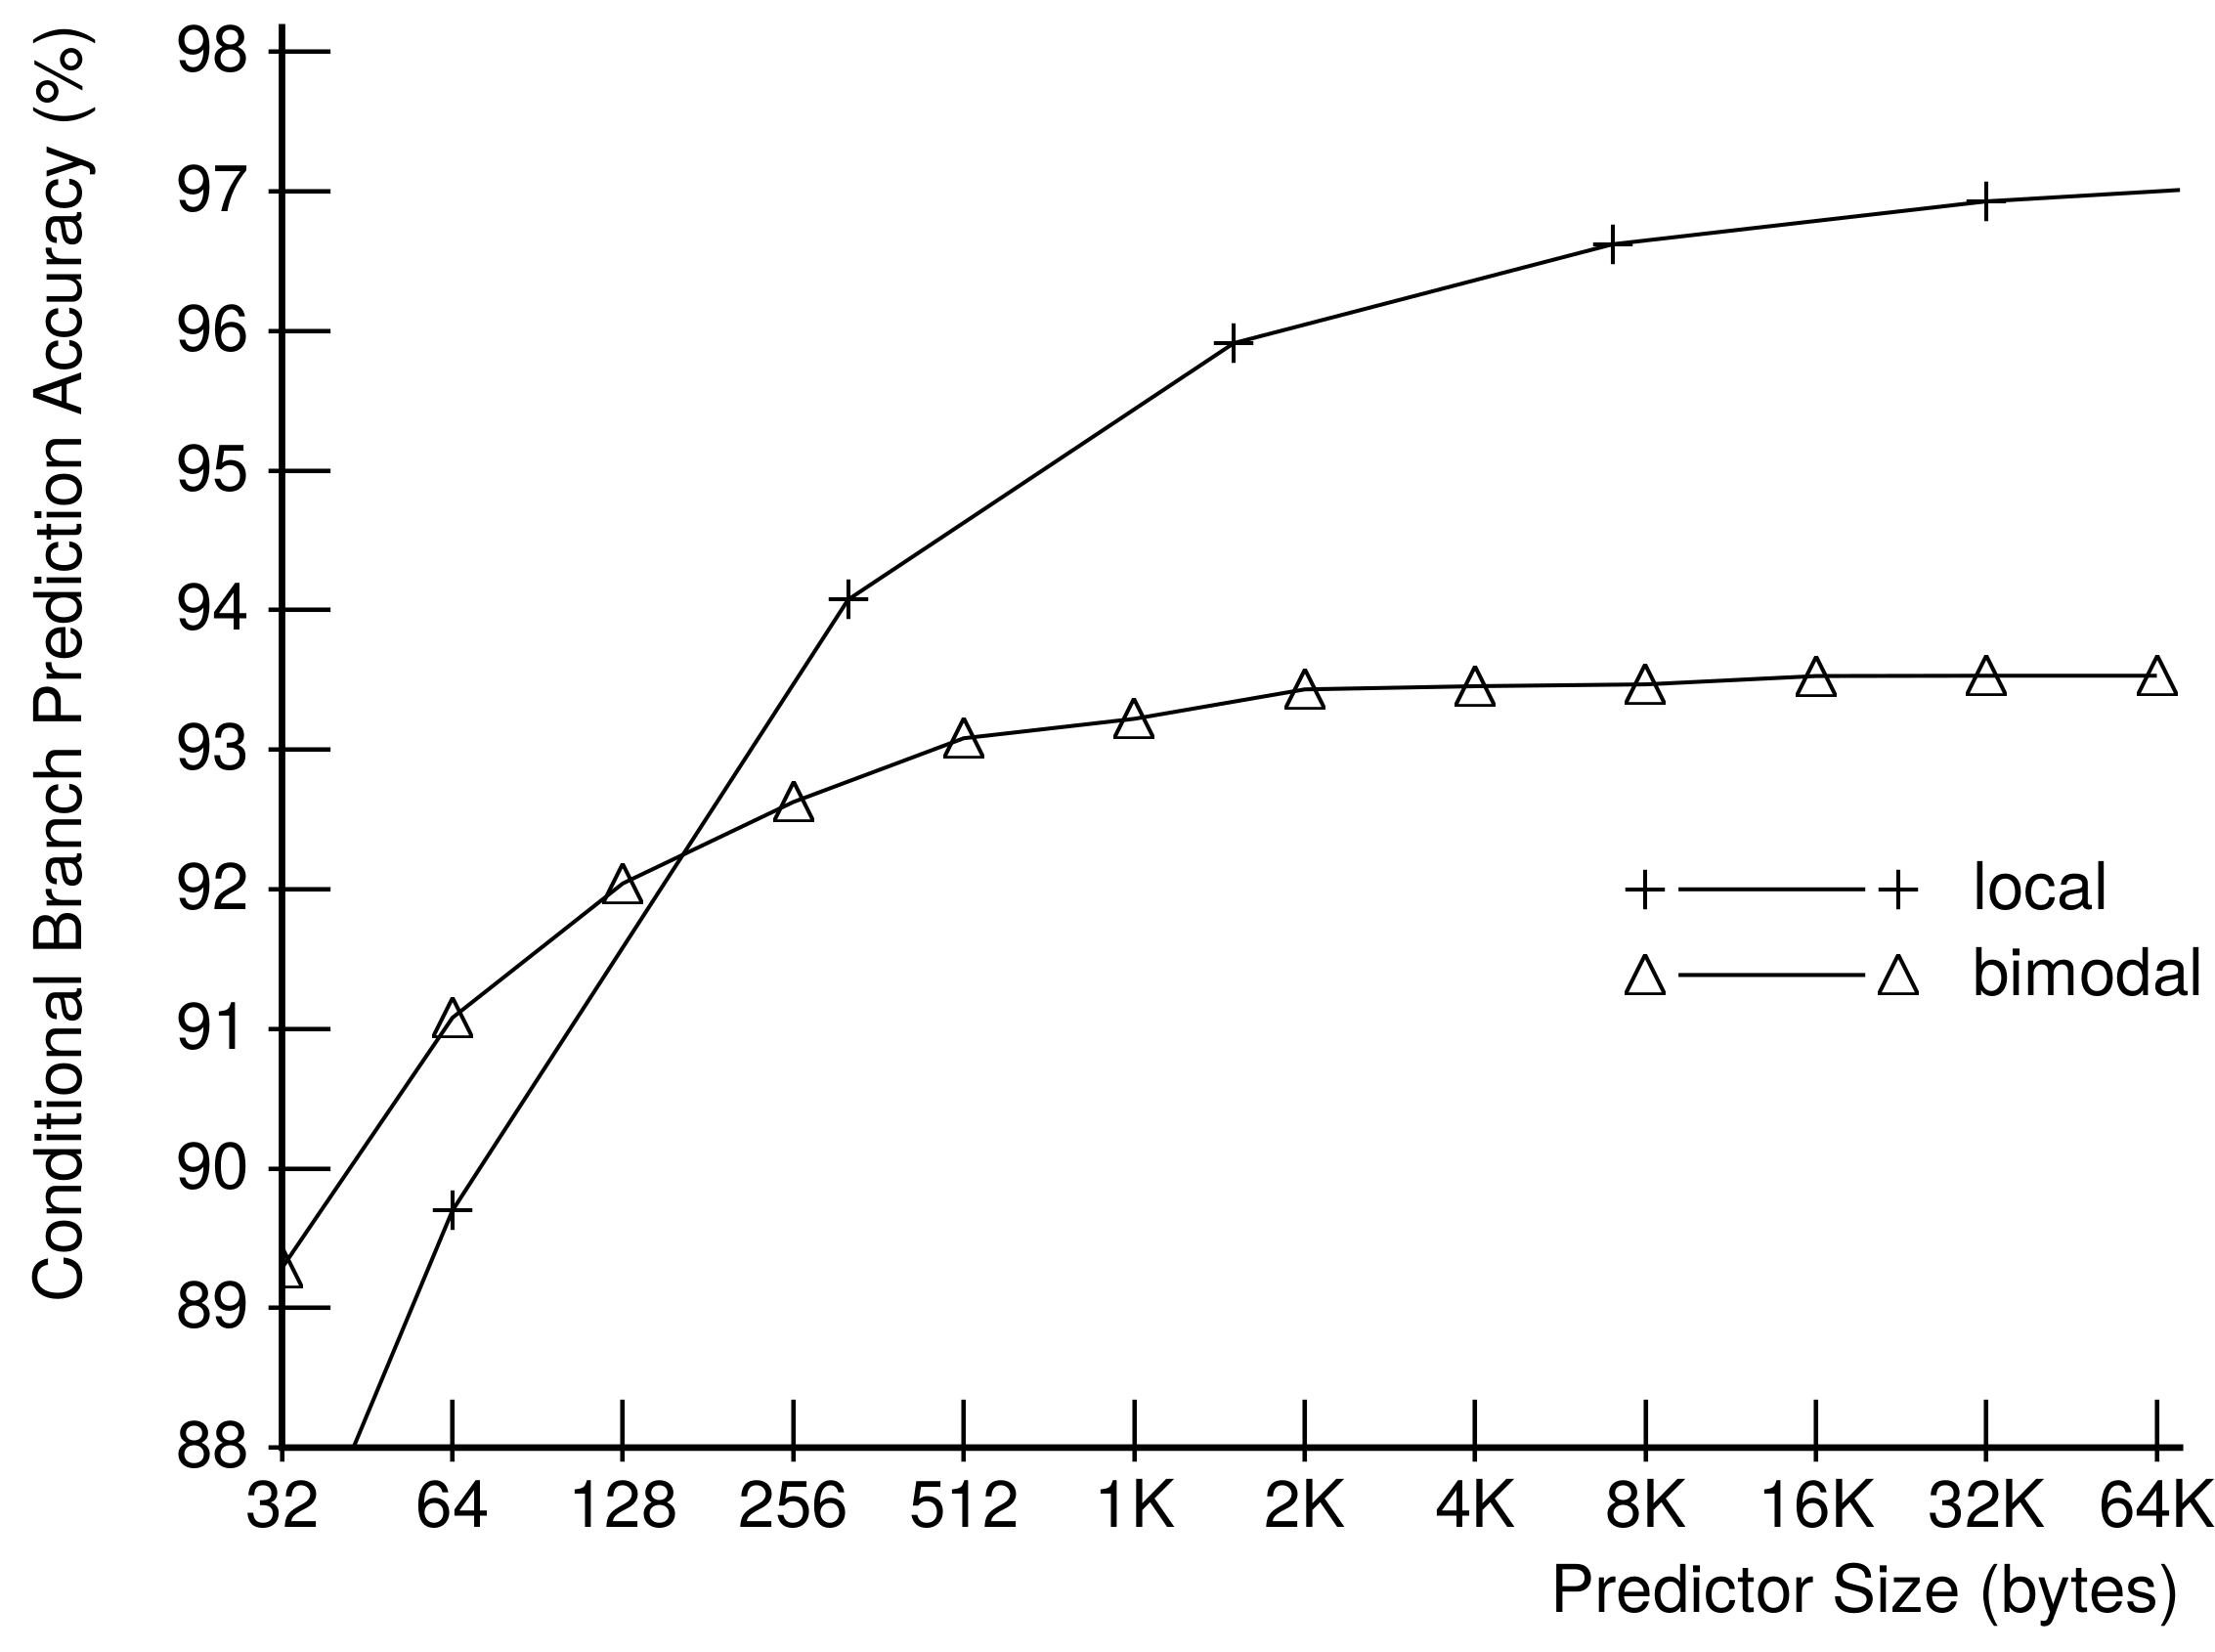
\includegraphics[height=0.8\textheight]{../bpred/mcf-local-bimodal}
\end{frame}

\begin{frame}{2-bit (bimodal) + local + global hist}
from McFarling, ``Combining Branch Predictors'' (1993)
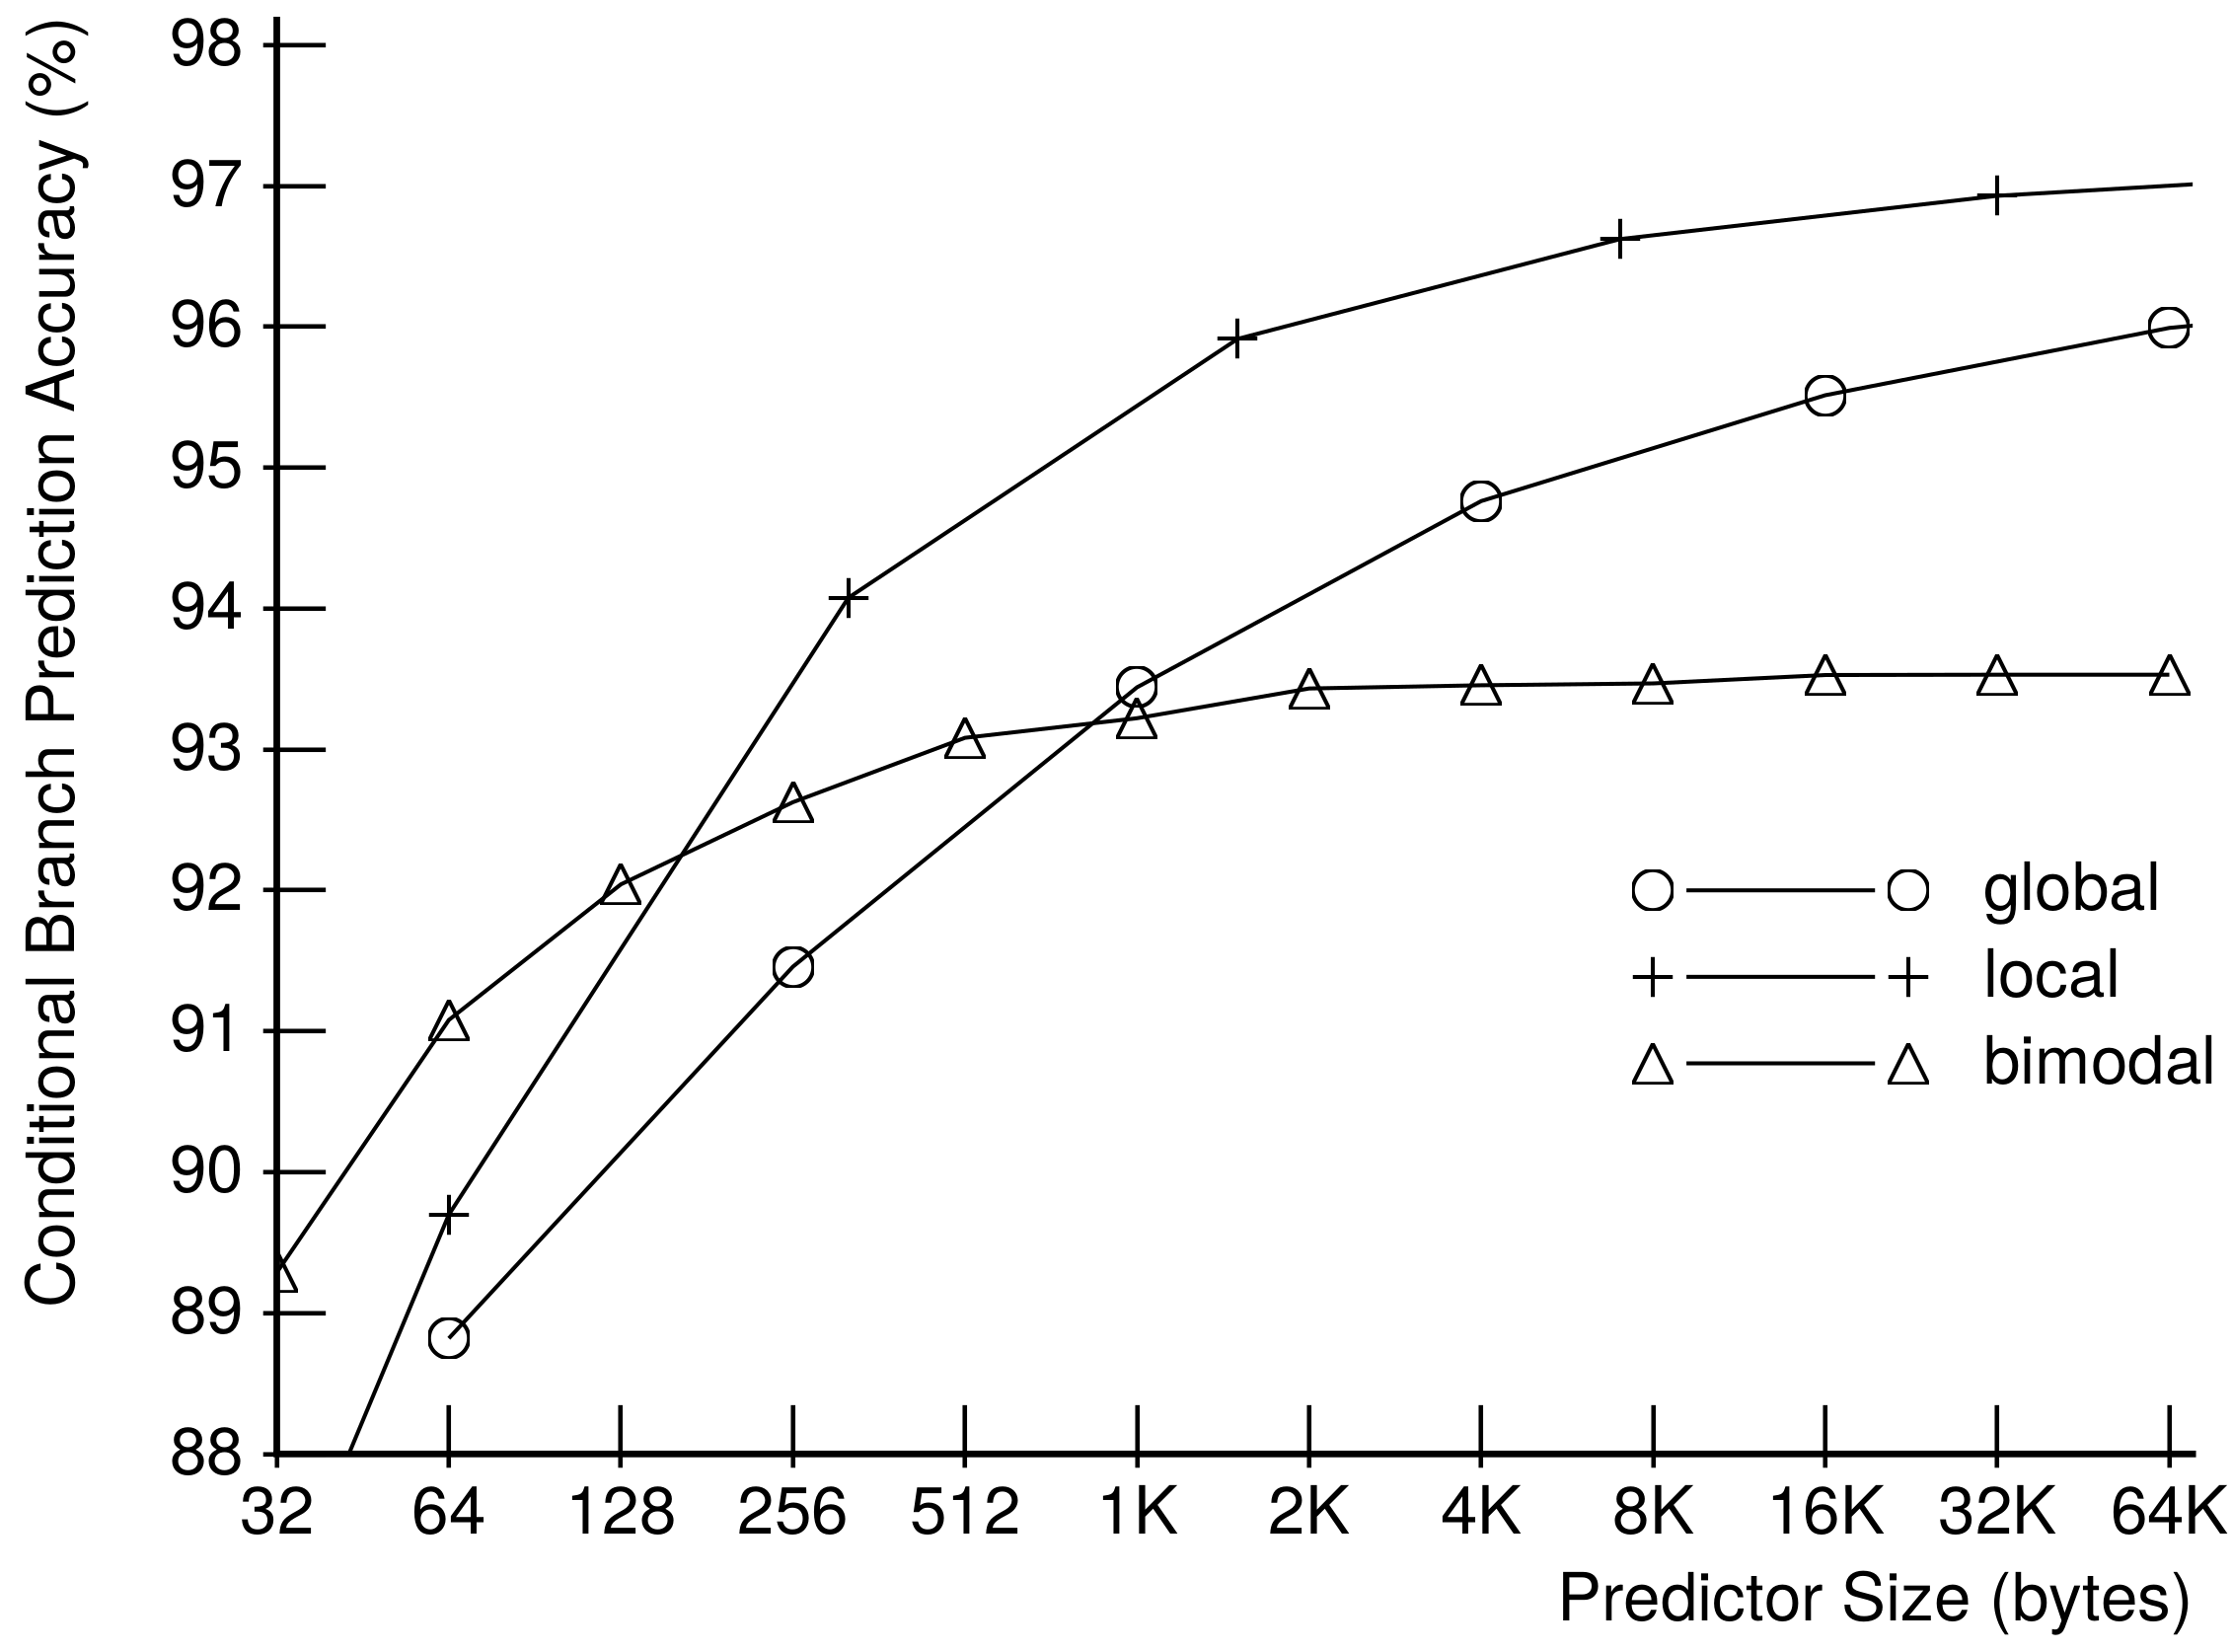
\includegraphics[height=0.8\textheight]{../bpred/mcf-local-bimodal-global}
\end{frame}

\begin{frame}{global + hash(global+PC) (gshare/gselect)}
from McFarling, ``Combining Branch Predictors'' (1993)
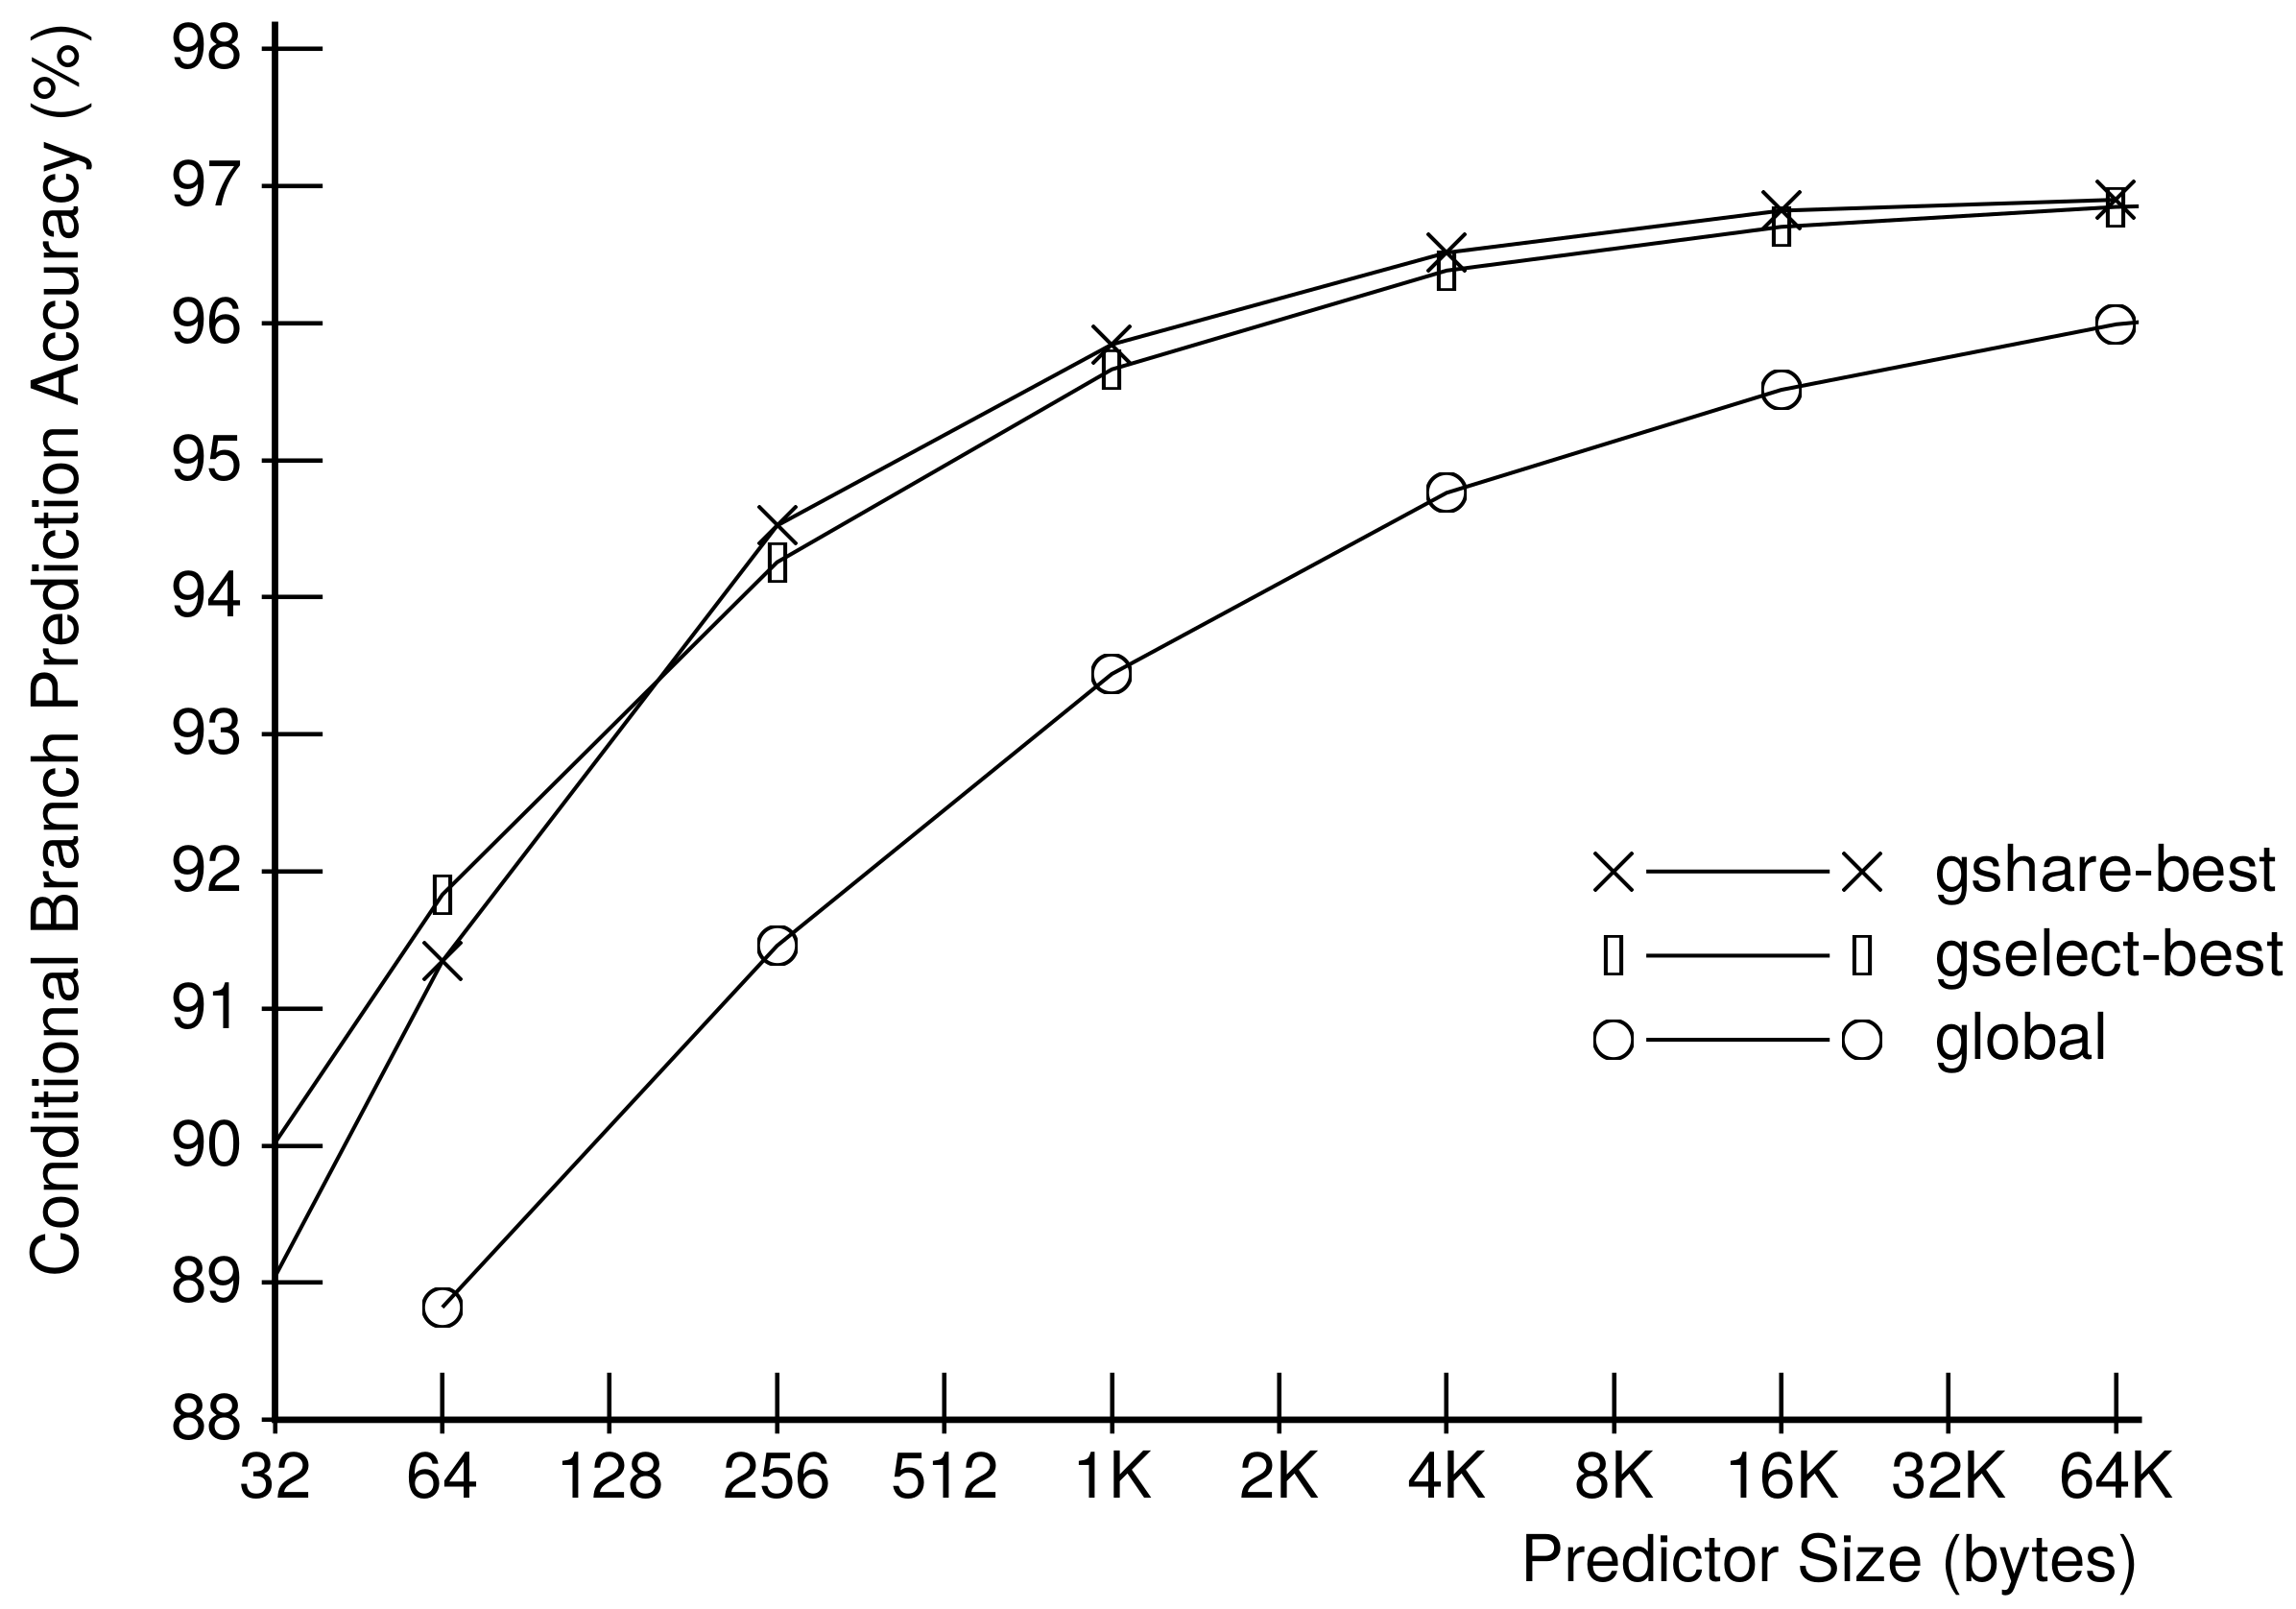
\includegraphics[height=0.8\textheight]{../bpred/mcf-global-gshare}
\end{frame}



\section{reversed engineering Haswell BP}
\begin{frame}{real BP?}
\begin{itemize}
\item details of modern CPU's branch predictors often not public
\item but\ldots
\vspace{.5cm}
\item Google Project Zero blog post with reverse engineered details
\item \scriptsize \url{https://googleprojectzero.blogspot.com/2018/01/reading-privileged-memory-with-side.html}
\item for RE'd BTB size:
\item \scriptsize \url{https://xania.org/201602/haswell-and-ivy-btb}
\end{itemize}
\end{frame}

\begin{frame}{reverse engineering Haswell BPs}
\begin{itemize}
\item branch target buffer
    \begin{itemize}
    \item 4-way, 4096 entries
    \item ignores bottom 4 bits of PC?
    \item hashes PC to index by shifting + XOR
    \item seems to store 32 bit offset from PC (not all 48+ bits of virtual addr)
    \end{itemize}
\item indirect branch predictor
    \begin{itemize}
    \item like the global history + PC predictor we showed, but\ldots
    \item uses history of recent branch addresses instead of taken/not taken
    \item keeps some info about last 29 branches
    \end{itemize}
\item what about conditional branches??? loops???
    \begin{itemize}
    \item couldn't find a reasonable source
    \end{itemize}
\end{itemize}
\end{frame}


\end{document}
